\documentclass[a4paper,12pt,oneside,onecolumn]{uerj}

\usepackage[brazil]{babel}  % adequacao para o portugues Brasil
\usepackage{cmap}           % Mapear caracteres especiais no PDF
\usepackage[utf8]{inputenc} % Determina a codificacao utiizada

\usepackage{array}
\usepackage{pgfplotstable}

\usepackage{caption}
\usepackage{subcaption}
\usepackage{pgfplots}
\usepackage{DejaVuSansMono}
\usepackage{listings}
\usepackage{makeidx}        % Cria o indice
\usepackage{hyperref}       % Controla a formacao do indice
\usepackage{indentfirst}    % Indenta o primeiro paragrafo de cada secao.
\usepackage{xcolor}
\usepackage{graphicx}       % Inclusao de graficos
\usepackage{amsmath,amssymb}        % pacote matemático
\usepackage{pdfpages}
\usepackage[top=3cm, bottom=2cm, left=3cm, right=2cm]{geometry}
\usepackage{chngcntr}

\usepackage[frame=no,gride=no,algline=yes,font=default]{uerjformat}
\usepackage[alf]{abntcite}
\newcommand{\formato}[1]{\begin{flushleft}{#1}\end{flushleft}}
\newcommand{\BibTeX}{{{Bib}}\TeX}

\logo{figures/logo_uerj_cinza.png}
\marcadagua{figures/marcadagua_uerj_cinza.png}{1}{160}{255}


\instituicao{Universidade do Estado do Rio de Janeiro}
            {Centro de Tecnologia e Ciências}
            {Instituto de Matemática e Estatística}
            {Departamento de Informática e Ciência da Computação}

\autor{Juan Pedro Alves}{Lopes}
\titulo{Uma Implementação de Expressões Regulares em Tempo Polinomial}

\orientador{Prof.} % rotulo
           {Paulo Eustáquio Duarte}{Pinto} % {nome}{sobrenome}
           {IME/DICC/UERJ} % afiliacao

\renewcommand{\coorientadornome}{Coorientadora}
\coorientador{Profª.} % rotulo
           {Maria Alice Silveira de}{Brito} % {nome}{sobrenome}
           {IME/DICC/UERJ} % afiliacao


\grau{Bacharel}
\curso{Informática e Tecnologia da Informação}

\local{Rio de Janeiro}   % cidade
\data{17}{Maio}{2013} % {dia}{mes}{ano}

% *****************************************************************************
% *****************************************************************************
% Configurações de aparência do PDF final
% *****************************************************************************
% *****************************************************************************

% alterando o aspecto da cor azul
%\definecolor{blue}{RGB}{41,5,195}

% informações do PDF
\hypersetup{
  %backref=true,
  %pagebackref=true,
  %bookmarks=true,                  % show bookmarks bar?
  pdftitle={\UERJtitulo},
  pdfauthor={\UERJautor},
  pdfsubject={\UERJpreambulo},
  pdfkeywords={Expressões Regulares}{Regex}{Autômatos Finitos},
  pdfproducer={LaTeX with class repUERJ}, % producer of the document
  pdfcreator={\UERJautor},
  colorlinks=true,                  % false: boxed links; true: colored links
  linkcolor=black,                   % color of internal links blue
  citecolor=black,                    % color of links to bibliography blue
  filecolor=black,                % color of file links magenta
  urlcolor=black,
  bookmarksdepth=4
}

\definecolor{mygray}{rgb}{0.5,0.5,0.5}
\definecolor{mygrayer}{rgb}{0.2,0.2,0.2}


\lstset{ %
  backgroundcolor=\color{white}, 
  basicstyle=\scriptsize\ttfamily,       
  captionpos=b,                 
  commentstyle=\color{mygray}, 
  deletekeywords={...},         
  escapeinside={\%*}{*)},       
  extendedchars=true,           
  keepspaces=true,              
  frame=single,
  keywordstyle=\bfseries\color{black},    
  morekeywords={*,...},         
  numbers=left,
  numbersep=5pt,                
  numberstyle=\scriptsize\color{mygray},
  rulecolor=\color{black},        
  showspaces=false,               
  showstringspaces=false,         
  showtabs=false,   
  firstnumber=1,     
  stepnumber=1,                   
  stringstyle=\color{mygrayer},    
  tabsize=2,    
  language=python,                 
  title=\lstname                 
}

\pgfplotsset{
	width=12cm,
	every axis legend/.append style={
		at={(0.5,1.03)},
		anchor=south
	}
}

\newtheorem{theorem}{Teorema}

\newenvironment{proof}[1][Demonstração]{\begin{trivlist}
\item[\hskip \labelsep \emph{#1}:]}{\end{trivlist}}

\newenvironment{definition}[1]{\noindent\hrulefill \begin{trivlist}
\item[\hskip \labelsep \textsc{#1}:]}{\end{trivlist}\noindent\hrulefill}


\newcommand{\qed}{\nobreak \ifvmode \relax \else
      \ifdim\lastskip<1.5em \hskip-\lastskip
      \hskip1.5em plus0em minus0.5em \fi \nobreak
      \vrule height0.75em width0.5em depth0.25em\fi}

\makeindex

\begin{document}

\counterwithout{lstlisting}{chapter}
\renewcommand*{\lstlistingname}{Listagem}
\renewcommand*{\lstlistlistingname}{Lista de listagens}
\frontmatter
\capa
\folhaderosto

%\includepdf{ficha_catalografica.pdf}

\begin{folhadeaprovacao}
  \assinatura{titulação membro1\\ afiliação1}
\end{folhadeaprovacao}

\pretextualchapter{Dedicatória}
  \vfill\vfill
    \hfill À minha esposa, Jacqueline.
  \vfill


\pretextualchapter{}

  \vfill\vfill\vfill\vfill
  \begin{flushright}
     Simplicity is a great virtue but it requires hard work\\
     to achieve it and education to appreciate it. And to \\
     make matters worse: complexity sells better.\\
    \textsl{-- Edsger W. Dijkstra}
  \end{flushright}
  \vfill

% ----------------------------------------------------------
% RESUMO
% ----------------------------------------------------------

\pretextualchapter{Resumo}

\refbibliografica

Na teoria, expressões regulares constituem uma notação para definir linguagens regulares em termos de operações recursivas simples. São equivalentes a autômatos finitos em seu poder expressivo. Na prática, apesar de serem ferramentas extremamente populares, as implementações modernas afastaram-se bastante da teoria que as originou. A maior parte das mudanças aconteceu para permiti-las alcançar um poder de expressão maior. Entretanto, esta conveniência trouxe o custo de tornar o \emph{match} um problema mais difícil computacionalmente do que a teoria descreve. Na maior parte das linguagens modernas o \emph{match} de \emph{regexes} (como são comumente conhecidas) é um problema NP-difícil. Além disso, por particularidades nas implementações, mesmo expressões que poderiam ser reconhecidas em tempo polinomial são resolvidas com soluções exponenciais. 

Neste trabalho são analisadas as armadilhas comuns no desenvolvimento de expressões regulares, realizando benchmarks entre diversas implementações populares, apontando funcionalidades que impediriam sua execução polinomial. É sugerida uma implementação simples e didática que garante tempo de execução polinomial, no pior caso.

\noindent {Palavras-chave}: Teoria da computação. Expressões regulares. Linguagens regulares. Autômatos finitos. Complexidade computacional. Algoritmos. NP-difícil.

% ----------------------------------------------------------
% Abstract
% ----------------------------------------------------------

\pretextualchapter{Abstract}

In theory, regular expressions are a notation to define regular languages in terms of simple recursive operations. They are equivalent to finite automata in its expressive power. In practice, modern regular expressions implementations deviated from the original theory. Most changes were made to allow them reach a greater expressive power. This convenience, however, came at the cost of making the match a harder problem than it could be. In most modern languages, the regex match is a NP-hard problem. Besides, the way they are implemented makes even expressions that could be recognized in polynomial time to be solved with exponential algorithms.

In this work, we analyze the common pitfalls in regular expressions development, measuring performance with benchmarks of the most popular implementations, pointing features that could not be implemented in polynomial time. Also it suggests a simple and didactic implementation which has superior worst-case performance than most popular implementations.

\noindent {Keywords}: Computation theory. Regular expressions. Regular languages. Finite automata. Computational complexity. Algorithms. NP-hard.

\listadefiguras
%\listadetabelas
\lstlistoflistings

\sumario

\mainmatter

%======================================================================================
\chapter{Introdução}
%======================================================================================

Neste capítulo serão apresentados a motivação, objetivos, e a estrutura do projeto.

%~~~~~~~~~~~~~~~~~~~~~~~~~~~~~~~~~~~~~~~~~~~~~~~~~~~~~~~~~~~~~~~~~~~~~~~
\section{Motivação}
%~~~~~~~~~~~~~~~~~~~~~~~~~~~~~~~~~~~~~~~~~~~~~~~~~~~~~~~~~~~~~~~~~~~~~~~

Expressões regulares fazem parte do ferramental da maioria das linguagens e plataformas de desenvolvimento modernas. Seu uso é bastante difundido na indústria para os mais variados fins, desde o reconhecimento de padrões, passando pela extração de símbolos para análise sintática de linguagens formais, até a sanitização de entradas do usuário para fins de segurança.

Seu extensivo uso vem precedido por uma forte base teórica na área de autômatos finitos, introduzida nos anos 40 por McCulloch e Pitts \cite{bib:McCulloch43} e formalizada na década seguinte por Kleene \cite{bib:Kleene56}.

Expressões regulares e autômatos finitos compartilham uma relação estreita. São equivalentes em poder expressivo, e a conversão do primeiro para o segundo é trivial, como pode ser visto na Figura \ref{fig:exemplo_automato}. Ken Thompson demonstrou isso em sua implementação no final dos anos 60 \cite{bib:Thompson68}, enquanto desenvolvia o editor de texto \emph{QED}. As mesmas expressões regulares foram, posteriormente, portadas para os mais conhecidos \emph{ed} e \emph{grep}, integrantes do sistema operacional Unix.

\begin{figure}[!htbp]
  \centering
  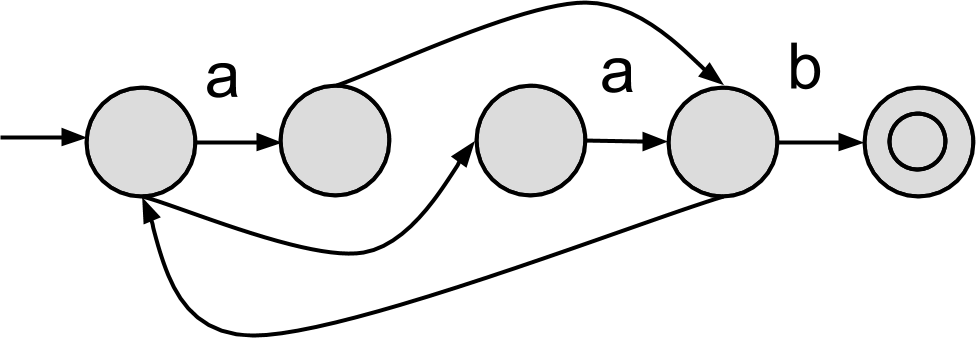
\includegraphics[scale=0.3]{figures/exemplo_automato.png}
  \caption{Exemplo de autômato para expressão regular $(a|a)^*b$}
  \label{fig:exemplo_automato}
\end{figure}

Desde então, conforme as implementações foram evoluindo, muitas funcionalidades foram adicionadas à linguagem de descrição de expressões regulares que as afastaram da teoria original. Enquanto originalmente descreviam linguagens estritamente regulares, a implementação mais difundida atualmente (\emph{PCRE}) é capaz não só de reconhecer qualquer linguagem livre de contexto, como também algumas sensíveis ao contexto. \cite{bib:Nikita12}

Uma das consequências mais notáveis desta evolução não planejada é que o reconhecimento de strings da linguagem, um problema com solução linear originalmente, ganhou soluções exponenciais em um grande número de implementações modernas, que inclui muitas das mais usadas. Talvez a funcionalidade mais perigosa neste sentido sejam as \emph{backreferences}, que não só impedem soluções polinomiais como tornam o problema de reconhecimento NP-difícil. Entretanto, mesmo nas expressões que poderiam ser reconhecidas estritamente com autômatos finitos, certas particularidades de implementação as tornam potencialmente exponenciais, no pior caso \cite{bib:Cox07}.

Linguagens como Python, Java e Ruby são amplamente utilizadas pelo mercado, porém suas bibliotecas-padrão implementam expressões regulares vulneráveis. A Figura \ref{fig:benchmark1} mostra o crescimento no tempo de execução entre suas implementações e a implementação proposta neste projeto (\emph{pyrex}).

\begin{figure}[!htbp]
\centering
\begin{tikzpicture}
	\begin{semilogyaxis}[xlabel=n, ylabel=tempo (s), legend columns=5, cycle list name=black white]
	\addplot table[x=n,y=pyrex] {benchmark/bench1.txt};
	\addplot table[x=n,y=python] {benchmark/bench1.txt};
	\addplot table[x=n,y=ruby] {benchmark/bench1.txt};
	\addplot table[x=n,y=java] {benchmark/bench1.txt};
	\legend{pyrex, python, ruby, java}
	\end{semilogyaxis}
\end{tikzpicture}
\caption{Tempo de execução (em escala logarítmica) para \emph{match} de $a^n$ contra $(a?a)^+b$}
\label{fig:benchmark1}
\end{figure}

Estas implementações tornam o uso de expressões regulares potencialmente inseguro em situações ora triviais. Um usuário mal intencionado pode ser capaz de forçar a execução de uma expressão com caráter exponencial para efetuar um ataque de negação de serviço em um servidor web. 

Por exemplo, ao permitir que entradas do usuário sejam interpretadas como expressões regulares, um usuário mal intencionado pode injetar a expressão $(a^a)^+b$, que por sua complexidade exponencial em implementações vulneráveis, ocuparia 100\% de uma CPU por um tempo virtualmente infinito. Vários ataques deste tipo podem causar instabilidade e queda do serviço web.

Muitas vezes a prevenção para esse tipo de ataque pode não ser trivial, e.g. em Java, onde métodos comumente usados sobre objetos oriundos da entrada do usuário, como \emph{replaceAll} e \emph{split}, da classe \emph{String} são implementados com expressões regulares vulneráveis a esse tipo de ataque.

Mesmo em casos onde o usuário mal intencionado não tem acesso à escrita de expressões regulares, um erro de programação pode deixar o sistema vulnerável a negação de serviço. Este problema torna-se especialmente notável pelo frequente compartilhamento em repositórios online, que contêm muitas expressões vulneráveis \cite{bib:Kirrage13,bib:Weidman10}. 

%~~~~~~~~~~~~~~~~~~~~~~~~~~~~~~~~~~~~~~~~~~~~~~~~~~~~~~~~~~~~~~~~~~~~~~~
\section{Objetivo}
%~~~~~~~~~~~~~~~~~~~~~~~~~~~~~~~~~~~~~~~~~~~~~~~~~~~~~~~~~~~~~~~~~~~~~~~

Este projeto tem dois objetivos principais. O primeiro é demonstrar através de testes pontuais e benchmarks os problemas fundamentais nas implementações de expressões regulares em diversas linguagens modernas, provando inclusive que o problema de reconhecimento de expressões regulares com \emph{backreferences} pertence à classe de problemas NP-difícil. O segundo objetivo é alcançar uma implementação didática e minimalista das expressões regulares, abordando as propostas por Kleene e utilizando o método descrito por Thompson para construção e simulação do autômato.

A implementação neste projeto não inclui certas funcionalidades comuns nos \emph{sabores} mais modernos de expressão regular. Algumas destas funcionalidades podem ser implementadas sem sacrificar eficiência de execução. Outras, introduzem certa complexidade, porém mantêm a execução do algoritmo polinomial. O restante, entretanto, não é possível implementar sem tornar o algoritmo exponencial no pior caso. Todas as funcionalidades intencionalmente excluídas serão listadas e propostas de soluções serão apresentadas quando cabível.

Pretende-se mostrar com esse projeto que o problema de reconhecimento de expressões regulares pode ser resolvido de maneira eficiente, mesmo com as implementações mais simples, desde que seja observada a base teórica que as deu origem.

%~~~~~~~~~~~~~~~~~~~~~~~~~~~~~~~~~~~~~~~~~~~~~~~~~~~~~~~~~~~~~~~~~~~~~~~
\section{Estrutura}
%~~~~~~~~~~~~~~~~~~~~~~~~~~~~~~~~~~~~~~~~~~~~~~~~~~~~~~~~~~~~~~~~~~~~~~~

O projeto está divido nos cinco capítulos, a saber:

\begin{description}

\item[Capitulo 2 -- Fundamentação Teórica:] base teórica por trás das expressões regulares, contando sua história, passando pelo método de construção do autômato de Thompson, e exibindo um algoritmo trivial (porém ineficiente) para sua solução.

\item[Capitulo 3 -- Implementação:] implementação apresentada neste trabalho, discutindo certos aspectos específicos desta implementação que não tenham sido abordados na parte de teoria. 

\item[Capitulo 4 -- Análise dos Resultados:] diferenças entre as implementações modernas e a implementação proposta neste trabalho. Neste capítulo é provada a pertinência em NP-difícil do \emph{match} de expressões com \emph{backreferences} e são mostrados benchmarks comparando as diversas implementações (inclusive a aqui apresentada), que evidenciam uma diferença fundamental na forma como o problema é abordado em cada uma delas. 

\item[Capitulo 5 -- Conclusão:] descrição das contribuições deste trabalho, bem como as dificuldades encontradas durante o projeto. Também serão listadas e descritas as funcionalidades não implementadas, possivelmente sugerindo formas eficientes de implementá-las, ou mesmo formas diferentes de simular o autômato que melhorem a eficiência geral da execução. 

\end{description}

%======================================================================================
\chapter{Fundamentação Teórica}\label{cap:theory}
%======================================================================================

Neste capítulo será introduzida um pouco da base teórica que guiou a implementação deste projeto.

%~~~~~~~~~~~~~~~~~~~~~~~~~~~~~~~~~~~~~~~~~~~~~~~~~~~~~~~~~~~~~~~~~~~~~~~
\section{Linguagens Formais}
%~~~~~~~~~~~~~~~~~~~~~~~~~~~~~~~~~~~~~~~~~~~~~~~~~~~~~~~~~~~~~~~~~~~~~~~

Linguagens formais é um tema que mistura elementos da ciência da computação, matemática e linguística. Seu papel na computação é fundamental pela relação de seus problemas com os descritos pela teoria da computação.

Uma \emph{linguagem formal} é um conjunto -- potencialmente infinito -- de \emph{palavras}, que por sua vez são combinações de elementos de um conjunto finito de símbolos chamado \emph{alfabeto}.

\subsection{Palavra}

Palavras são combinações entre os elementos de um alfabeto. Por exemplo, com um alfabeto $\Sigma = \{0, 1\}$, é possível formar palavras que representam números binários.

Uma palavra é representada pelos símbolos que a compõem. Logo, 01101 é uma palavra formada pelos símbolos do alfabeto descrito anteriormente. Uma palavra especial, denotada $\epsilon$ (às vezes $\lambda$) representa uma palavra vazia.

Dado um alfabeto com $k$ símbolos, é possível formar até $k^n$ palavras de tamanho $n$. Logo, existem

\begin{equation*}
	\mathlarger \sum^{n}_{i=0} k^i = \frac{k^{n+1}-1}{k-1}
\end{equation*}

palavras de até $n$ caracteres num alfabeto com $k$ símbolos.

O conjunto formado por todas as palavras de um alfabeto é infinito, porém enumerável. Uma possível estratégia é numerá-los primeiro por seu tamanho, então por sua ordem lexicográfica.

A operação básica entre palavras é a \emph{concatenação}. Por exemplo, 

\begin{alignat*}{3}
w_1 = aaa &, w_2=bbb  &\Rightarrow w_1w_2 &= aaabbb \\
w_1 = aaa &, w_2=\epsilon  &\Rightarrow w_1w_2 &= aaa \\
w_1 = \epsilon &, w_2=bbb  &\Rightarrow w_1w_2 &= bbb \\
\end{alignat*}

Concatenação é associativa, então 

\begin{equation*}
(w_1w_2)w_3 = w_1(w_2w_3),
\end{equation*}

porém não comutativa, logo

\begin{equation*}
w_1w_2 \neq w_2w_1.
\end{equation*}

\subsection{Linguagem}

Linguagens são conjuntos de palavras sobre algum alfabeto. A mesma notação de conjuntos é utilizada para elas. Por exemplo, $A \cup B$ representa a linguagem formada pela união de todas as palavras de A e B, assim como $w \in A$ é uma proposição que afirma que a palavra $w$ está presente na linguagem A.

É possível concatenar linguagens. Dadas linguagens $L_1$ e $L_2$,

\begin{equation*}
	L_1L_2 = \{w_1w_2 \mid w_1 \in L_1, w_2 \in L_2\}
\end{equation*}

E.g.: se $A = \{a, aa\}$ e $B = \{b, bb\}$, então $AB = \{ab, aab, abb, aabb\}$.


Com base na concatenação, uma operação importante em linguagens é o fecho Kleene (ou fecho de concatenação, $L^*$), que pode ser definido recursivamente como:

\begin{equation*}
	L^0 = \{\epsilon\}
\end{equation*}
\begin{equation*}
	L^i = L^{i-1}L
\end{equation*}
\begin{equation*}
	L^* = \bigcup_{i \in \mathbb{N}} L^i
\end{equation*}

E.g.: se $A = \{a, aa\}$, então $A^* = \{\epsilon, a, aa, aaa, \ldots\}$.

Existem duas formas principais para se definir linguagens formais. \emph{Gramáticas gerativas}, que geram palavras da linguagem a partir de sistemas de reescrita; e \emph{Autômatos}, que reconhecem palavras da linguagem. 

Além destas, existem diversas outras formas de definir linguagens. As próprias expressões regulares denotam linguagens formais da classe das regulares. Outra forma bastante é comum é através da sintaxe de geração de conjuntos, e.g. $L=\{a^n \mid n \in \mathbb{N}\}$.

%~~~~~~~~~~~~~~~~~~~~~~~~~~~~~~~~~~~~~~~~~~~~~~~~~~~~~~~~~~~~~~~~~~~~~~~
\section{Gramáticas Gerativas}
%~~~~~~~~~~~~~~~~~~~~~~~~~~~~~~~~~~~~~~~~~~~~~~~~~~~~~~~~~~~~~~~~~~~~~~~

Uma das formas de representar linguagens formais é através de gramáticas gerativas. O termo ``gramática formal'' é comumente utilizado para referir-se a elas. No entanto, existem outras formas de representar gramáticas formais além deste.

Gramáticas gerativas são sistemas de reescrita, i.e. a partir de um símbolo inicial, é possível usar as regras de reescrita para produzir todas as palavras de uma linguagem. Esta operação é, de certa forma, o problema dual de reconhecer uma palavra como parte da linguagem através de um autômato \cite{bib:Ruohonen09}.

Uma gramática gerativa é formada por uma tupla $G = (N, \Sigma, P, S)$. Onde:

\begin{itemize}
    \item N é o conjunto de símbolos não terminais. Eles não fazem parte da linguagem original, então precisam ser sempre substituídos para alcançar uma palavra válida na linguagem.
    \item $\Sigma$ é o conjunto de símbolos terminais da linguagem. Também conhecido como alfabeto.
    \item P é o conjunto de regras de produção, geralmente na forma $\alpha \rightarrow \beta \mid \alpha, \beta \in (N \cup \Sigma)*$.
    \item S é o símbolo inicial do sistema de reescrita. $S \in N$.
\end{itemize}

Um exemplo de gramática é a que define cadeias da forma $a^nb^n, n>0$:

\begin{equation*}
	G = ({\{S\}, \{a,b\}, P, S})
\end{equation*}

Onde P é definido por:

\begin{equation*}
	S \rightarrow aSb
\end{equation*}
\begin{equation*}
	S \rightarrow ab
\end{equation*}

Iniciando do símbolo S, é possível começar com a regra $ab$ ou $aSb$. A primeira já forma uma palavra na linguagem que queremos descrever ($ab$), a segunda possui um símbolo não terminal. A partir dele é possível gerar as palavras na linguagem: $aabb$, $aaabbb$, etc...

Perceba que na gramática todas as regras do lado esquerdo possuem apenas um símbolo não terminal. Se fôssemos escrever uma gramática para cadeias na forma $a^nb^nc^n$, precisaríamos de uma gramática mais rebuscada:

\begin{equation*}
	G = (\{S, T\}, \{a,b,c\}, P, S)
\end{equation*}

Onde P é definido por:

\begin{equation*}
	S \rightarrow aTSc
\end{equation*}
\begin{equation*}
	S \rightarrow abc
\end{equation*}
\begin{equation*}
	Ta \rightarrow aT
\end{equation*}
\begin{equation*}
	Tb \rightarrow bb
\end{equation*}

O fato desta gramática definir sequências de símbolos à esquerda com mais de um símbolo a torna especial. Segundo a hiearquia de Chomsky, a primeira gramática é livre de contexto, enquanto a segunda é sensível ao contexto.

%~~~~~~~~~~~~~~~~~~~~~~~~~~~~~~~~~~~~~~~~~~~~~~~~~~~~~~~~~~~~~~~~~~~~~~~
\section{Hierarquia de Chomsky}
%~~~~~~~~~~~~~~~~~~~~~~~~~~~~~~~~~~~~~~~~~~~~~~~~~~~~~~~~~~~~~~~~~~~~~~~

Segundo Noam Chomsky \cite{bib:Chomsky57}, uma gramática formal pode ser classificada em um dos quatro tipos baseados em sua capacidade expressiva:

\begin{description}
    \item[Tipo 0:] gramáticas recursivamente enumeráveis (ou irrestritas)
    \item[Tipo 1:] gramáticas sensíveis ao contexto
    \item[Tipo 2:] gramáticas livres de contexto
    \item[Tipo 3:] gramáticas regulares
\end{description}

Como pode ser visto no diagrama da Figura~\ref{fig:chomsky}, cada conjunto é propriamente incluso no seu conjunto superior na hierarquia. Há entretanto uma ligeira exceção no caso das gramáticas sensíveis ao contexto, pois estas não podem gerar a string $\epsilon$, enquanto as livres de contexto podem. Gramáticas livres de contexto que geram $\epsilon$ constituem a única exceção da pertinência às gramáticas sesíveis ao contexto.

\begin{figure}[!htbp]
  \centering
  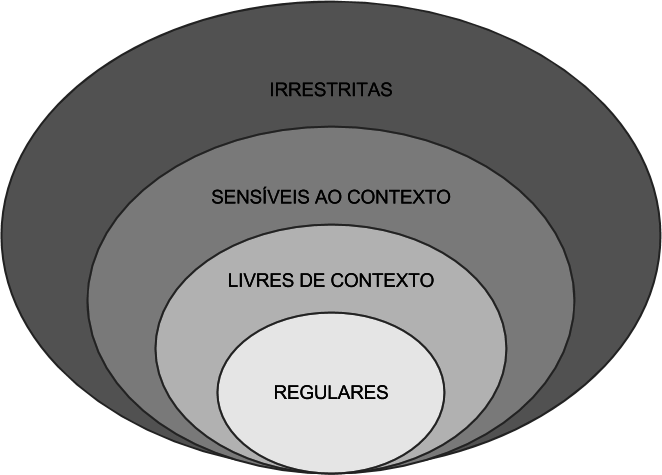
\includegraphics[scale=0.5]{figures/chomsky.png}
  \caption{Representação da inclusão de conjuntos na hiearquia de Chomsky}
  \label{fig:chomsky}
\end{figure}

\subsection{Gramáticas Regulares}

Gramáticas regulares são aquelas cujas regras de produção são na forma $S \rightarrow a$ ou $S \rightarrow aT$, onde \emph{S} e \emph{T} são não-terminais e \emph{a} é um terminal na linguagem. Estas gramáticas são equivalentes em poder de expressão a \emph{autômatos finitos}. 

Opcionalmente a regra $S \rightarrow aT$ pode ser substituída por $S \rightarrow Ta$, mas nunca as duas podem ocorrer na mesma gramática. Se a primeira ocorre, a gramática é conhecida como \emph{linear à direita}. Caso contrário, é \emph{linear à esquerda}. \cite{bib:Chomsky58}

Exemplos de linguagens regulares incluem: endereços de email, repetição de caracteres ($a^n$), repetição independente de dois caracteres ($a^nb^m$).

\subsection{Gramáticas Livres de Contexto}

Gramáticas livres de contexto são aquelas onde todas as regras de produção são do tipo $S \rightarrow \gamma$, onde \emph{S} é um não-terminal e $\gamma$ é uma sequência composta por terminais e não-terminais. 

Isto na prática significa que a substituição de um não-terminal é sempre feita independente do contexto onde é encontrado. Gramáticas deste tipo são equivalentes em poder expressivo a \emph{autômatos de pilha}. Elas compõem a base teórica para a maioria das linguagens de programação. 

Entre alguns exemplos clássicos de linguagens livres de contexto figuram: parênteses aninhantes, repetição condicionada de dois caracteres ($a^nb^n$), expressões aritméticas.

\subsection{Gramáticas Sensíveis ao Contexto}
Gramáticas sensíveis ao contexto são aquelas onde aparecem regras de produção do tipo $\alpha S\beta\rightarrow \alpha\gamma\beta$, em que $\alpha$, $\gamma$ e $\beta$ são sequências compostas por terminais e não-terminais. Elas diferem das gramáticas livres de contexto por definir -- exatamente -- contexto para que um não-terminal S seja substituído por uma sequência $\gamma$. 

Apesar dessas exigências de contexto, as cadeias dessa classe de linguagens ainda são passíveis de ser reconhecidas com o emprego de um \emph{autômato linearmente limitado}. 

Exemplos de liguagens sensíveis ao contexto: \emph{squares} (\emph{DogDog, CatCat, WikiWiki...}), \emph{matching triplets} ($a^nb^nc^n$).

\subsection{Gramáticas Recursivamente Enumeráveis}

As gramáticas para as linguagens recursivamente enumeráveis não apresentam restrições em suas regras, o que faz com que essas linguagens sejam também chamadas de ``sem restrição". Portanto, qualquer sequência de terminais e não-terminais $\alpha$ pode ser substituída por outra $\beta$. Cadeias de linguagens assim são reconhecíveis por uma \emph{máquina de Turing}. 

Diferente dos tipos anteriores, quando é submetida a reconhecimento uma cadeia que não faça parte da linguagem, não há garantia de parada da máquina, definindo o que é chamado de \emph{conjunto semi-decidível}.

Um dos exemplos mais notáveis de linguagens recursivamente enumeráveis que não são sensíveis ao contexto é a sintaxe de templates do C++ \cite{bib:Veldhuizen03}.

\subsection{Tabela de Referência}

É possível resumir os tipos de linguagens da hierarquia de Chomsky numa tabela de referência quanto às máquinas que as reconhecem e os tipos de regras das gramáticas que as geram.

\begin{center}
	\begin{tabular}{ c | c | c | c }
		 & {\bf Linguagem} & {\bf Máquina} & {\bf Regras} \\
		\hline 
		0 & Recursivamente enumerável & Máquina de Turing 			 & 
			$\alpha \rightarrow \beta$ \\ 
		1 & Sensível ao contexto 		& Autômato limitado linearmente & 
			$\alpha S\beta\rightarrow \alpha\gamma\beta$\\ 
		2 & Livre de contexto 			& Autômato de pilha 			 & 
			$S \rightarrow \gamma$\\ 
		3 & Regular 					& Autômato finito 				 &
			$S \rightarrow aT$ ou $S \rightarrow a$\\ 
	\end{tabular}
\end{center}

%~~~~~~~~~~~~~~~~~~~~~~~~~~~~~~~~~~~~~~~~~~~~~~~~~~~~~~~~~~~~~~~~~~~~~~~
\section{Expressões Regulares}
%~~~~~~~~~~~~~~~~~~~~~~~~~~~~~~~~~~~~~~~~~~~~~~~~~~~~~~~~~~~~~~~~~~~~~~~

Expressões regulares são sequências de caracteres que denotam linguagens regulares. Definimos uma expressão regular (ER), em um alfabeto $\Sigma$, através de seis expressões regulares primitivas ER1 $\ldots$ ER6. É dito que $\alpha$ é uma expressão regular se e somente se ela puder ser determinada a partir destas primitivas, a seguir:

\begin{description}
    \item[ER1] $\emptyset$ denota a linguagem vazia.
    \item[ER2] $\epsilon$ denota a linguagem que contém apenas cadeia vazia.
    \item[ER3] Todo caractere $a \in \Sigma$ é uma expressão regular.
    \item[ER4] Se $\alpha$ e $\beta$ são expressões regulares que denotam $L_\alpha$ e $L_\beta$ respectivamente, $\alpha|\beta$ denota a linguagem $L_\alpha \cup L_\beta$.
    \item[ER5] Se $\alpha$ e $\beta$ são expressões regulares que denotam $L_\alpha$ e $L_\beta$ respectivamente, $\alpha\beta$ denota a linguagem $L_\alpha L_\beta$.
    \item[ER6] Se $\alpha$ é uma expressão regular que denota $L_\alpha$, $\alpha^*$ denota a linguagem $L_\alpha^*$.
\end{description}

Perceba que é possível definir outros operadores comuns, como $?$ e $^+$. Mas é possível fazê-lo a partir das operações descritas acima. O operador $e_1?$ pode ser definido como a alternância $e_1|\epsilon$. O operarador $e_1^+$ pode ser definido como $e_1e_1^*$.

Outros operadores sobre caracteres como o $.$ (qualquer caractere) e as classes de caractere (e.g. $[a-zA-Z]$) são trivialmente implementados usando alternação de expressões.

A precedência natural dos operadores, da mais fraca para a mais forte, é: alternância, concatenação, repetição. Assim, uma expressão como $ab|cd^*$ é interpretada como exibido na Figura~\ref{fig:abcd_parse_tree}.

\begin{figure}[!htbp]
  \centering
  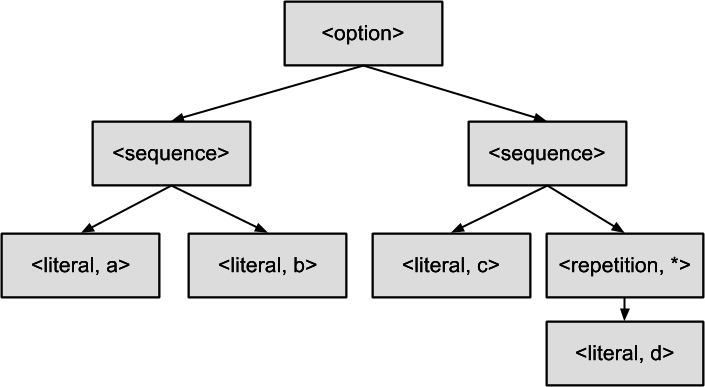
\includegraphics[scale=0.4]{figures/abcd_parse_tree.png}
  \caption{Árvore de avaliação para expressão $ab|cd^*$}
  \label{fig:abcd_parse_tree}
\end{figure}

É possível agrupar sub-expressões utilizando parênteses, tal qual é feito com expressões aritméticas. Assim $a(b|c)d^*$ tem um sentido completamente diferente de $ab|cd^*$.

Estas operações, utilizando somente três operadores, definem inequivocamente expressões regulares. É possível denotar qualquer linguagem regular utilizando apenas estes operadores. Mais importante: é teoricamente possível reconhecer qualquer cadeia desta linguagem com apenas uma passagem pela entrada (sem \emph{backtracking}). 

Novas implementações de expressões regulares adicionaram novos operadores que tornam a sintaxe mais concisa. Porém, essas adições normalmente não alteram o poder expressivo das \emph{regexes}, sendo encontradas adições que aumentam o poder expressivo, como é o caso das \emph{backreferences}, que permitem o reconhecimento de algumas linguagens não-regulares. \emph{Backreferences} consistem em referências \emph{submatches} reconhecidas anteriormente.

Pode ser observado o exemplo de uma linguagem composta por palavras repetidas, como \emph{DogDog} ou \emph{CatCat}, para o qual é possível definir uma expressão regular $/(.^*)\backslash 1/$ que reconhece esta linguagem. $\backslash 1$ instrui o motor de reconhecimento a esperar uma nova palavra exatamente igual à obtida pelo reconhecimento do primeiro grupo $(.^*)$. Esta linguagem é sensível ao contexto, i.e. não apenas fica fora do conjunto das linguagens regulares, como também não é uma linguagem livre de contexto.

Tal poder expressivo tem seu preço. O reconhecimento de \emph{backreferences} é um problema NP-difícil, logo, os melhores algoritmos conhecidos ainda têm pior caso exponencial. É possível, porém, escrever algoritmos polinomiais para expressões que não fazem uso de \emph{backreferences}.

Para suportar \emph{backreferences}, a implementação mais comum consiste em \emph{backtracking} com memória das capturas anteriores, o que impede a utilização de \emph{memorização}, técnica que poderia tornar polinomial a complexidade deste tipo de implementação. Mais detalhes sobre os tipos de implementação são discutidos na Seção~\ref{sec:simulacao}, na Página~\pageref{sec:simulacao}.

Uma outra solução seria utilizar duas implementações, uma garantidamente polinomial (para casos simples) e outra possivelmente exponencial (para casos mais complexos), porém este tipo de solução exige grande esforço de engenharia para manter concordantes os resultados das duas implementações.

%~~~~~~~~~~~~~~~~~~~~~~~~~~~~~~~~~~~~~~~~~~~~~~~~~~~~~~~~~~~~~~~~~~~~~~~
\section{Autômatos Finitos}
%~~~~~~~~~~~~~~~~~~~~~~~~~~~~~~~~~~~~~~~~~~~~~~~~~~~~~~~~~~~~~~~~~~~~~~~

Autômatos finitos representam um modelo matemático de computação. Eles representam máquinas abstratas constituídas de um número finito de estados. Formalmente, autômatos finitos são uma tupla $M = (Q, \Sigma, q_0, \delta, A)$, onde:

\begin{itemize}
    \item Q é o conjunto de estados do autômato. Sempre finito.
    \item $\Sigma$ é o alfabeto da linguagem reconhecida pelo autômato.
    \item $q_0$ é o estado inicial do autômato. $q_0 \in Q$.
    \item $\delta$ é a função de transição, que mapeia cada $(q_i, a) \in Q \times \Sigma$ a um subconjunto de Q. Se esse subconjunto tem apenas zero ou um elemento, o autômato é \emph{deterministico}, caso contrário, ele é \emph{não-determinístico}. Cabe notar que para cada autômato não-determinístico, há um autômato determinístico equivalente \cite{bib:Rabin59}.
    \item A é o conjunto de estados de aceite. $A \subseteq Q$.
\end{itemize}

Por exemplo:

\begin{figure}[!htbp]
  \centering
  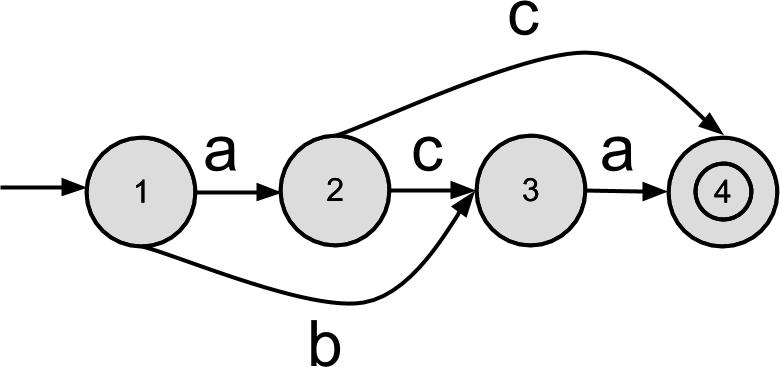
\includegraphics[scale=0.3]{figures/exemplo_automato_numerado.png}
  \caption{Diagrama de estados de um autômato não-determinístico}
  \label{fig:exemplo_automato_numerado}
\end{figure}

O autômato na Figura~\ref{fig:exemplo_automato_numerado} pode ser descrito por $M=(\{1,2,3,4\}, \{a,b,c\}, 1, \delta, \{4\})$, onde $\delta$ é definida pela tabela de transições:

\begin{center}
	\begin{tabular}{ c || c | c | c }
		{\bf $\delta$} & {\bf a} & {\bf b} & {\bf c} \\
		\hline 
		\hline 
		1 & 2 & 3 &  \\ 
		\hline 
		2 &   &   & 3, 4 \\ 
		\hline 
		3 & 4 &   &  \\ 
		\hline 
		4 &   &   &  \\ 
	\end{tabular}
\end{center}

Este autômato é \emph{não determinístico}, pois se a máquina reconhecedora estiver no  estado 2 e for lido o símbolo $c$, esse par de parâmetros (estado, entrada) causam na função de transição um resultado com dois estados alternativos, o 3 ou o 4, caracterizando um indeterminismo.

Autômatos finitos não-determinísticos também aceitam um tipo de entrada especial $\epsilon$, que não consome caracteres da entrada, como pode ser visto na Figura~\ref{fig:exemplo_automato_epsilon}. Perceba que este autômato \emph{não é equivalente} ao definido anteriormente. Ele aceita uma palavra $b$ que o primeiro não aceita.

\begin{figure}[!htbp]
  \centering
  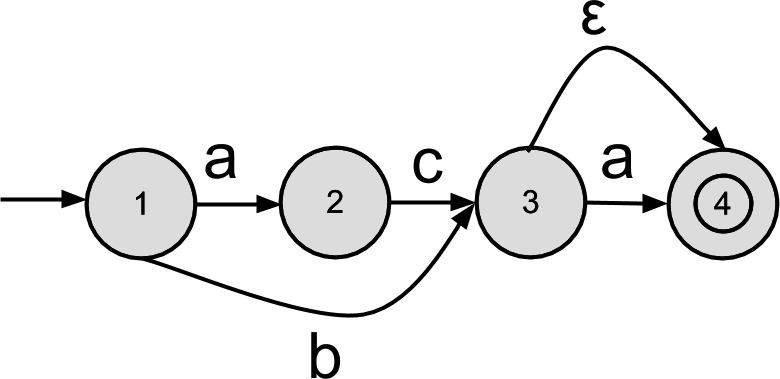
\includegraphics[scale=0.3]{figures/exemplo_automato_epsilon.png}
  \caption{Diagrama de estados de um autômato não-determinístico com entrada $\epsilon$}
  \label{fig:exemplo_automato_epsilon}
\end{figure}


Autômatos finitos podem ser construídos para reconhecer cadeias das linguagens regulares. Assim, o processo de reconhecimento de uma cadeia submetida a um autômato desse tipo termina em estados de aceite se e somente se essa cadeia fizer parte da linguagem para a qual o autômato foi construído.

O autômato descrito na Figura~\ref{fig:exemplo_automato_epsilon}, por exemplo, reconhece uma linguagem finita definida por $L = \{ac, aca, b, ba\}$. A linguagem que um autômato finito reconhece é \emph{sempre regular}. E \emph{toda linguagem regular} pode ser reconhecida com autômatos finitos \cite{bib:Kleene56}.

%~~~~~~~~~~~~~~~~~~~~~~~~~~~~~~~~~~~~~~~~~~~~~~~~~~~~~~~~~~~~~~~~~~~~~~~
\section{Método de Construção de Thompson}
%~~~~~~~~~~~~~~~~~~~~~~~~~~~~~~~~~~~~~~~~~~~~~~~~~~~~~~~~~~~~~~~~~~~~~~~

Pela sinergia entre expressões regulares e autômatos finitos e pela facilidade de lidar com cada um deles em situações específicas, é útil poder converter entre um e outro. Ken Thompson \cite{bib:Thompson68} descreveu um método para construir autômatos a partir de expressões regulares.

Na época em que foi escrito, o artigo descrevia como gerar código de máquina para um IBM 7094. Isto era necessário por restrições de hardware da época. Hoje não é mais estritamente necessário. Este trabalho irá se limitar a descrever como construir o autômato a partir da expressão regular.

O método consite em construir o autômato recursivamente através da análise da árvore sintática da expressão, procedimento que precisa ser efetuado antes do começo da construção do autômato. No artigo original de Thompson, este passo era feito construindo a expressão em notação \emph{infixa}. Entretanto, para permitir extensibilidade do formato da expressão, iremos definir completamente a gramática da expressão regular que aceitaremos.

\subsection{Analise sintática}

O primeiro passo para a construção do autômato é analisar sintaticamente a expressão, construindo a árvore sintática. 

Podemos definir uma gramática gerativa simples pela notação EBNF (\emph{Extended Backus–Naur Form}) que representa a linguagem formada pelas expressões regulares.

\begin{verbatim}
<option>     ::= <sequence> { "|" <sequence> }*
<sequence>   ::= <repetition> { <repetition> }*
<repetition> ::= <primary> { "*" | "?" | "+" }*
<primary>    ::= "." | <literal> | "(" <option> ")"
\end{verbatim}

Assim, a expressão pode ser facilmente analisada. Por exemplo, a expressão $(a|a)^+b$ seria avaliada como a árvore descrita na Figura~\ref{fig:aab_parse_tree}.

\begin{figure}[!htbp]
  \centering
  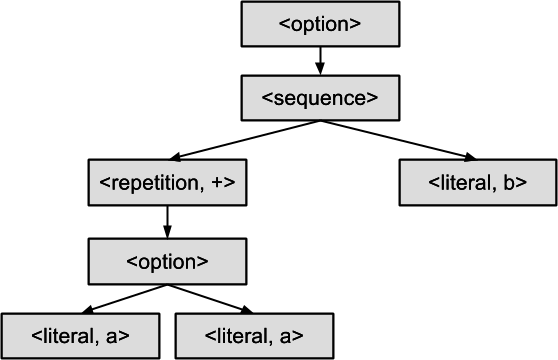
\includegraphics[scale=0.5]{figures/aab_parse_tree.png}
  \caption{Árvore de avaliação para expressão $(a|a)^+b$}
  \label{fig:aab_parse_tree}
\end{figure}

Utilizando a EBNF, esta árvore pode ser produzida por diversos tipos de ferramentas geradoras de compiladores presentes em várias linguagens. Exemplos notáveis incluem o YACC (\emph{Yet Another Compiler Compiler}), o JAVACC (\emph{Java Compiler Compiler}) e o ANTLR (\emph{ANother Tool for Language Recognition}).

Com esta árvore de avaliação é possível fazer a conversão para o autômato de forma bastante trivial, como será discutido nas próximas seções.

\subsection{Notação}
\label{sec:Notacao}

Iremos assumir uma notação diferente para representação do autômato, que irá facilitar a construção. Para fins de praticidade, todo estado $q_i \in Q$ será de um entre três tipos possíveis:

\begin{enumerate}
    \item Estado de \emph{consumo},  com apenas uma transição $(a \in \Sigma, S \in N)$.
    \item Estado de \emph{decisão}, com uma transição $\epsilon$ para um estado ou duas transições $\epsilon$ para estados distintos.
    \item Estado de aceite, com nenhuma transição
\end{enumerate}

A Figura~\ref{fig:nova_notacao} mostra como podem ser representados os estados desta nova notação no diagrama de estados.

\begin{figure}[!htbp]
  \centering
  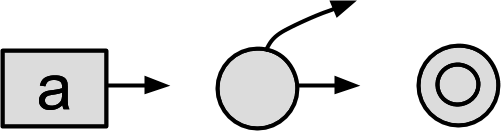
\includegraphics[scale=0.5]{figures/nova_notacao.png}
  \caption{Representação de estados na nova notação}
  \label{fig:nova_notacao}
\end{figure}

Esta representação facilita a visualização por omitir as transições $\epsilon$ e ressaltar a diferença entre os estados de consumo e os estados de decisão. Um exemplo de conversão para a nova notação pode ser visto na Figura~\ref{fig:exemplo_nova_notacao}.

\begin{figure}[!htbp]
  \centering
  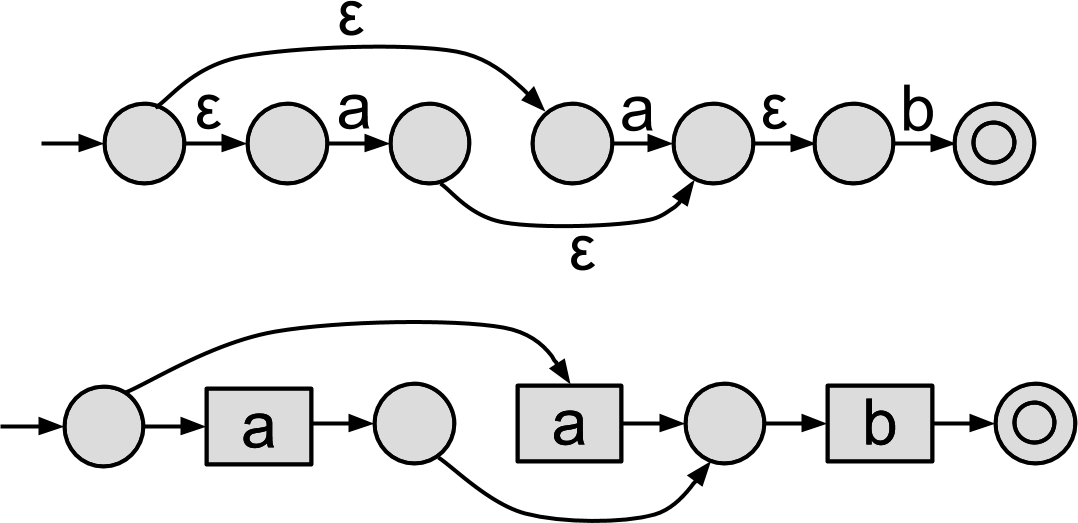
\includegraphics[scale=0.25]{figures/exemplo_nova_notacao.png}
  \caption{Mesmo autômato representado com as duas notações}
  \label{fig:exemplo_nova_notacao}
\end{figure}

\subsection{Construção}

A construção do autômato se dá pela conversão recursiva de cada um dos nós na árvore por uma construção de autômato predeterminada. Cada uma destas construções tem apenas um estado de entrada e todas as transições que não apontem para um nó dentro da própria construção, apontam para um único nó de saída.

Em uma implementação otimizada, este passo pode ser substituído por geração de código de máquina (como no artigo original). Entretanto, para fins didáticos, abordaremos algumas representações úteis do autômato gerado.

A tabela a seguir mostra a conversão para cada tipo de nó. Para fins de notação, as letras maiúsculas representam autômatos complexos produzidos em passos anteriores, mas que seguem a mesma regra definida no parágrafo anterior.

\begin{center}
	\begin{tabular}{ c | c | c }
		{\bf Tipo} & {\bf Expressão} & {\bf Construção} \\
		\hline
		\hline
		Literal & $a$ & 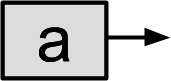
\includegraphics[scale=0.25]{figures/thompson_literal.png} \\ 
		\hline
		Sequência & $ST$ & 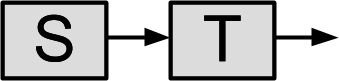
\includegraphics[scale=0.25]{figures/thompson_sequence.png} \\ 
		\hline
		Opção & $S|T$ & 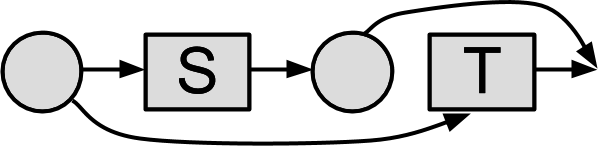
\includegraphics[scale=0.25]{figures/thompson_option.png} \\ 
		\hline
		Kleene+ & $S+$ & 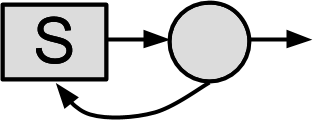
\includegraphics[scale=0.25]{figures/thompson_plus.png} \\ 
		\hline
		Opcional & $S?$ & 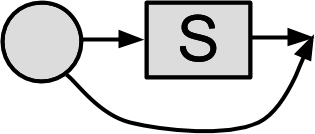
\includegraphics[scale=0.25]{figures/thompson_question.png} \\ 
		\hline
		Kleene* & $S*$ & 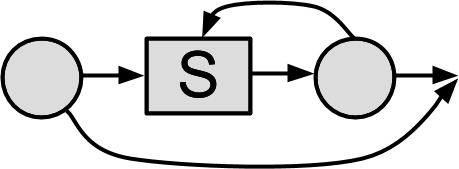
\includegraphics[scale=0.25]{figures/thompson_kleene.png} \\ 
		\hline
	\end{tabular}
\end{center}

Para converter um autômato usando estas regras, basta percorrer a árvore de avaliação de baixo para cima, inicialmente transformando todos os literais e recursivamente usando-os como insumo para os nós superiores. A Figura~\ref{fig:exemplo_automato_completo} mostra um exemplo de conversão utilizando a expressão $(a|a)^+b$.

\begin{figure}[!htbp]
  \centering
  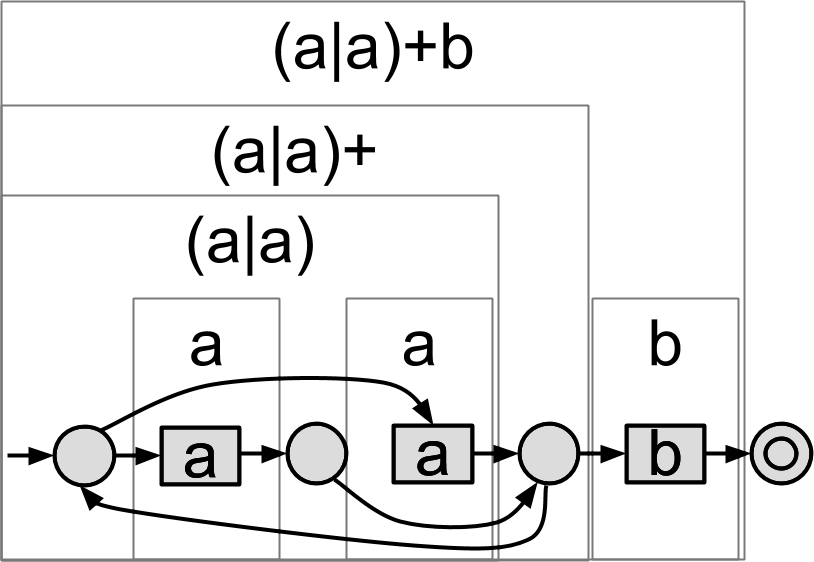
\includegraphics[scale=0.33]{figures/exemplo_automato_completo.png}
  \caption{Exemplo completo de autômato para a expressão $(a|a)^+b$}
  \label{fig:exemplo_automato_completo}
\end{figure}

Uma das vantagens desta forma de construir é que ela pode ser escrita como uma sequência de instruções para serem interpretadas por uma máquina virtual. Cada um dos três tipos de estados definidos pela notação na seção anterior podem ser substituídos por uma entre três instruções. Estados de consumo como instruções \emph{CONSUME}, estados de decisão como instruções \emph{JUMP} e estados de aceite como instruções \emph{MATCH}.

Por exemplo, o autômato representado pela Figura~\ref{fig:exemplo_automato_completo} pode ser reescrito como as instruções:

\nopagebreak 
\begin{verbatim}
0000: JUMP (1, 3)
0001: CONSUME a
0002: JUMP (2,)
0003: CONSUME a
0004: JUMP (1, -4)
0005: CONSUME b
0006: MATCH!
\end{verbatim}

As instruções \emph{JUMP} são as que representam o não-determinismo destes autômatos, pois ao serem executadas, podem desviar para qualquer um dos rótulos para os quais apontam. Existem diversas formas de simular a execução desses programas não-determinísticos usando uma máquina de Turing determínistica. E é exatamente neste ponto onde a maior parte das implementações torna-se exponencial desnecessariamente.

%~~~~~~~~~~~~~~~~~~~~~~~~~~~~~~~~~~~~~~~~~~~~~~~~~~~~~~~~~~~~~~~~~~~~~~~
\section{Simulação do Autômato}\label{sec:simulacao}
%~~~~~~~~~~~~~~~~~~~~~~~~~~~~~~~~~~~~~~~~~~~~~~~~~~~~~~~~~~~~~~~~~~~~~~~

Simular a execução de um autômato não-determinístico utilizando uma máquina determinística é um problema por si só complicado. Pode existir um número exponencial de caminhos possíveis num autômato não-determinístico \cite{bib:Rabin59}.

Dentre as opções para simulação da execução do autômato, estão:

\begin{itemize}
    \item \emph{Backtracking}: tentar todos os caminhos possíveis, voltando para a última escolha feita em caso de falha.
    \item \emph{Backtracking com memorização}.
    \item \emph{Conversão para DFA}: converter para um autômato determinístico antes de executar.
    \item \emph{Simulação paralela}: simular a execução de todos os estados simultaneamente.
	\item \emph{Conversão preguiçosa para DFA}: semelhante a execução paralela, mas construindo um cache dos estados alcançados
\end{itemize}

Cada uma destas opções tem características próprias. Suas vantagens e desvantagens serão discutidas separadamente.

\subsection{Backtracking}

Backtracking é talvez a forma mais trivial de implementar a simulação de autômatos não determinísticos. Consiste basicamente em diante de várias opções escolher uma delas, mas manter uma pilha de escolhas feitas para retroceder e escolher novamente caso não tenha sucesso.

\emph{Vantagem}: Este método é o que oferece a possibilidade de uma implementação mais fácil, pois como a chamada de subrotinas na maior parte das linguagens já utiliza uma pilha para a alocação do seu registro de ativação, uma simples recursão é o suficiente para implementar esta técnica.

\emph{Desvantagem}: Pela natureza do autômato, cada escolha pode gerar vários fluxos independentes, então uma sequência de n escolhas (assumindo que sejam binárias) pode gerar até $2^n$ fluxos diferentes. Além disso, esta técnica requer múltiplas passagens pela mesma string, o que é trivial se ela estiver em memória, mas complicado se estiver vindo de um fluxo de rede ou pipes do sistema. E por fim, a pilha reservada para chamadas de métodos é compartilhada com outros recursos e limitada em diversos ambientes, impossibilitando, por exemplo, o reconhecimento de strings muito grandes.

\subsection{Backtracking com Memorização}

O maior problema de usar backtracking talvez seja a quantidade de fluxos diferentes que a implementação pode alcançar. Entretanto, para o problema de reconhecimento, a resposta é invariante se definirmos em termos de $s_i, q_j$ tal que $s_i \in S, q_j \in Q$, onde $S$ é a entrada e $Q$ o conjunto de estados do autômato.

Definindo assim, se $n = |S|, m = |Q|$, então existem apenas $n \times m$ possíveis configurações para o problema, que podem ser devidamente memorizadas. Então um problema que era $O(2^n)$ torna-se $O(n\times m)$.

\emph{Vantagem}: Esta técnica é tão fácil de implementar quanto o backtracking puro e tem complexidade bem menor.

\emph{Desvantagem}: Ainda é necessário passar multiplas vezes pela mesma string. E a pilha ainda pode ser um fator limitante.

\subsection{Conversão para DFA}

Autômatos finitos determinísticos são muito mais fáceis de simular, visto que são mais próximos dos computadores que conhecemos atualmente. 

É sabido que autômatos finitos determinísticos (DFA) e não-determinísticos (NFA) são equivalentes em termos de poder expressivo. É possível converter entre um e outro com métodos conhecidos. NFAs tem baixa complexidade de memória, mas são mais custosos em tempo de execução. DFAs, entretanto permitem uma execução mais rápida ao custo de uma alta complexidade de memória. 

Um NFA com m estados, quando convertido para um DFA pode ter ate $2^m$ estados. Em termos de memória utilizada, NFAs são exponencialmente mais expressivos que DFAs \cite{bib:Calabro05}. Entretanto, DFAs tem execução com menor complexidade que NFAs. Para uma entrada com n caracteres, NFAs podem ser simulados em $O(n \times m)$, enquanto DFAs em $O(m)$.

A conversão entre os dois se dá através do algoritmo conhecido como \emph{Rabin-Scott powerset construction} \cite{bib:Rabin59}. Este algoritmo consiste basicamente em simular a execução paralela do autômato para todas as entradas possíveis.

\emph{Vantagem}: Depois de construído o DFA, ele pode ser usado para reconhecer qualquer string em $O(m)$.

\emph{Desvantagem}: A construção do DFA tem complexidades de tempo e espaço exponenciais. E é bem mais complexa do que o backtracking puro.

\subsection{Simulação paralela}

Uma forma de simular a execução de autômatos é, sempre que confrontado com uma decisão, escolher as duas opções simultaneamente, e manter fluxos paralelos sendo executados. 

Inicialmente, pode parecer que esta solução leve a um conjunto de até $2^n$ fluxos executando simultaneamente, porém, como um autômato tem um número finito de estados, existem no máximo $m$ fluxos simultâneos para cada caractere. Eventualmente, múltiplas decisões podem colidir num mesmo estado, eliminando assim o caráter exponencial da avaliação. Assim, para uma entrada com n caracteres avaliada contra um autômato de m estados, no pior caso, a complexidade de tempo é de $O(n \times m)$.

O objetivo é que durante a execução, seja lido um caractere por vez. Então, antes de cada execução é preciso avaliar todas as transições $\epsilon$ e deixar todos os fluxos em espera posicionados em estados do tipo \emph{consumo}.

A Figura~\ref{fig:nfa_simultaneo} mostra a execução do autômato gerado para a expressão regular $(a|a)^+b$ contra a entrada $aa$.

\begin{figure}[!htbp]
  \centering
  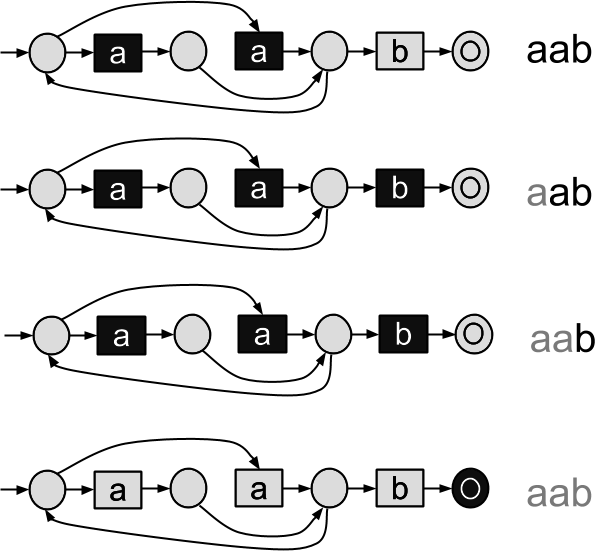
\includegraphics[scale=0.5]{figures/nfa_simultaneo.png}
  \caption{Passos do reconhecimento da expressão $(a|a)^+b$ contra a entrada \emph{aab}}
  \label{fig:nfa_simultaneo}
\end{figure}

\emph{Vantagem}: Tem tempo de execução polinomial ($O(n \times m)$). Só precisa ler a entrada uma vez. Não requer uso de pilha.

\emph{Desvantagem}: Precisa de memória adicional para guardar os estados executados ($O(m)$). Em comparação com execução com DFA puro, é mais lento.

\subsection{Conversão preguiçosa para DFA}

O maior perigo da conversão completa para DFA é o potencial explosivo que a geração do autômato determinístico tem. Até $2^n$ estados podem ser gerados, e tempo proporcional a isso será gasto. Por outro lado, a simulação parelela parece gastar uma quantidade linear de memória e tempo polinomial para simular o autômato.

Para a maior parte das aplicações práticas, dificilmente a quantidade de estados no DFA será tão grande. Por isso, uma aproximação combinada entre as duas abordagens poderia trazer vantagens.

Durante a simulação paralela, os estados ativados simultaneamente correspondem exatamente a um estado no respectivo DFA. Ao realizar cache destes estados (porém mantendo uma política de gerência de memória, descartando os mais antigos) a implementação estará mantendo a complexidade de execução da simulação paralela, porém aumentando as chances de eventualmente gerar o DFA completamente.

\emph{Vantagem}: Tem tempo de execução linear no caso médio ($O(n)$). Só precisa ler a entrada uma vez. Não requer uso de pilha.

\emph{Desvantagem}: Pior caso ainda é $O(n \times m)$. Precisa de memória adicional para guardar os estados executados e o cache de estados do DFA. Implementação consideravelmente mais complexa.

%======================================================================================
\chapter{Implementação}\label{cap:implementation}
%======================================================================================

Neste capítulo será apresentada a implementação da biblioteca \emph{PyRex} (expressões regulares em Python). A implementação na íntegra pode ser visualizada no Apêndice~\ref{app:full_source}.

Neste projeto o objetivo era alcançar uma implementação completamente polinomial para expressões regulares. Alcançado o primeiro objetivo, a implementação foi focada na simplicidade. Foram evitados truques de implementação que a tornassem mais rápida em detrimento da legibilidade. Todas as escolhas foram para reduzir a complexidade da implementação. Mesmo assim, o algoritmo utilizado foi eficiente o bastante para atingir o objetivo inicial.

A linguagem escolhida para implementar o projeto foi Python. É uma linguagem de máquina virtual, tal qual o Java. Entretanto, sua máquina virtual não tem as otimizações em tempo de execução que as implementações mais famosas de Java têm. Além disso, a resolução dinâmica de tipos a faz ter uma performance inferior à de outras linguagens com resolução estática de tipos. 

Mesmo assim, pela reduzida quantidade de caracteres especiais em sua sintaxe, os programas escritos nela são em geral mais legíveis e simples. Por isso, toda a implementação do PyRex tem menos de 90 linhas de código (contando as em branco) e menos de 3KB. Esta implementação abrange desde a análise sintática da expressão regular até a simulação do autômato retornando, inclusive, a região do reconhecimento da expressão.

O projeto foi implementado utilizando apenas as bibliotecas padrão disponíveis no Python 2.7, porém ele também funciona no Python 3.0 e superiores.

\section{Funcionalidades Implementadas}

Foi escolhido um conjunto de funcionalidades que fosse capaz de mostrar o ponto de falha das implementações modernas de expressões regulares e ainda assim ser simples o suficiente para ter uma implementação que pudesse ser explicada em alguns minutos.

Assim, foi implementado o reconhecimento de:

\begin{itemize}
    \item Literais (e.g. $a$)
    \item Sequências (e.g. $ab$)
    \item Alternâncias (e.g. $ab|cd$)
    \item Agrupamentos (e.g. $a(bc)d$)
    \item Expressão opcional (e.g. $a?$)
    \item Kleene* (e.g. $a^*$)
    \item Kleene+ (e.g. $a^+$)
\end{itemize}

Estas funcionalidades são bem próximas às definidas por Thompson \cite{bib:Thompson68} em seu artigo e permitem denotar inequivocamente linguagens regulares.

\section{Estrutura do Código}

O código está dividido em basicamente duas partes: um \emph{parser} e um \emph{matcher}.

O \emph{parser} é responsável por receber uma string com a expressão regular, analisá-la sintaticamente e retornar um objeto (o \emph{matcher}) capaz de reconhecer strings que façam parte da linguagem regular definida.

O \emph{matcher} contém informações do autômato gerado e funções que sabem simular a execução do autômato. Ele é implementado como uma classe Python com um método \emph{match}, além da sobrecarga do operador \emph{\_\_repr\_\_} do Python, que provê uma visualização útil do objeto em tempo de depuração.

O uso desta biblioteca se dá pela compilação do autômato usando a função \emph{rex} e a posterior avaliação de strings usando o método \emph{match} da classe \emph{Machine}. Um exemplo de uso pode ser visto na listagem~\ref{lst:usage_example}.

\vspace{0.5cm}
\begin{lstlisting}[caption={Exemplo de uso da biblioteca PyRex},label=lst:usage_example]
import pyrex
machine = pyrex.rex('a(ab)+')
print machine.match('aabab')
\end{lstlisting}

O retorno da chamada da função match pode ser tanto uma tupla com dois elementos (índices de início e final do match) ou uma referência nula (\emph{None} em Python). No exemplo da Listagem~\ref{lst:usage_example}, o retorno seria uma tupla $(0, 5)$, indicando que o match começa no índice 0 da string e termina no índice 4. Perceba que a tupla denota um intervalo aberto à direita.

\section{Análise sintática}

Análise sintática é feita pela função \emph{rex}. Ela implementa um parser recursivo descendente rudimentar. A BNF está descrita abaixo:

\begin{verbatim}
<option>     ::= <sequence> { "|" <sequence> }*
<sequence>   ::= { <repetition> }*
<repetition> ::= <primary> { "*" | "?" | "+" }*
<primary>    ::= "." | <literal> | "(" <option> ")"
\end{verbatim}

É importante chamar a atenção para o detalhe da regra \emph{sequence} que permite strings vazias. Esta é uma mudança que permite strings vazias como expressão regular (o que é útil em alguns casos). Entretanto, esta mesma mudança permite expressões regulares do tipo $a||b$. O que não chega a constituir um erro. A Listagem~\ref{lst:sequence} mostra a implementação desta regra.

\vspace{0.5cm}
\begin{lstlisting}[caption={Implementação da regra \emph{sequence}},label=lst:sequence]
def sequence():
    e = []
    while tokens and tokens[0] not in '|)':
        e += repetition()
    return e
\end{lstlisting}

A implementação é bem simples, usa uma instância da classe \emph{deque} como buffer de tokens e chamadas recursivas para implementar as regras. Para cada uma das quatro regras defindas pela BNF, há um método aninhado em \emph{rex} para representá-la.

O tratamento de erros é simples porém eficiente. Sempre que um caractere não esperado é encontrado na entrada, ele é reportado. Um dos mecanismos pode ser observado no código principal do parser (Listagem~\ref{lst:main_parser}), onde após consumir todos os caracteres possíveis, se ainda existirem remanescentes na entrada, uma exceção é lançada.

\vspace{0.5cm}
\noindent\begin{minipage}{\textwidth}
\begin{lstlisting}[caption={Exemplo de tratamento de erros no parser},label=lst:main_parser]
e = option()
if tokens: 
    raise Exception('Not expected: "{}"'.format(''.join(tokens)))

return Machine(e)
\end{lstlisting}
\end{minipage}

\section{Representação}

Durante o parse, a expressão regular é transformada numa representação do autômato relacionado. Este autômato é representado como um \emph{array de objetos}, onde cada posição do array representa um estado do autômato.

Como definido na Seção~\ref{sec:Notacao} (Página~\pageref{sec:Notacao}), a notação utilizada neste autômato prevê três tipos de estado: consumo, decisão e aceite. Estados de consumo são representados pelo caractere que consomem. Estados de decisão são representados por uma tupla de inteiros que informam quantos estados à frente ou atrás deve-se `pular'. Estados de aceite não precisam de representação, pois sempre ocorrem no final do autômato (segundo esta notação).

A Figura~\ref{fig:exemplo_automato_puro} e as listagens \ref{lst:automaton_array} e \ref{lst:automaton_instr} representam a expressão regular $(a|a)^+b$. Apenas a forma em array é armazenada na instância da classe Machine para execução. Entretanto, a forma em instruções pode ser gerada através do método \emph{\_\_repr\_\_} da mesma classe.

\begin{figure}[!htbp]
  \centering
  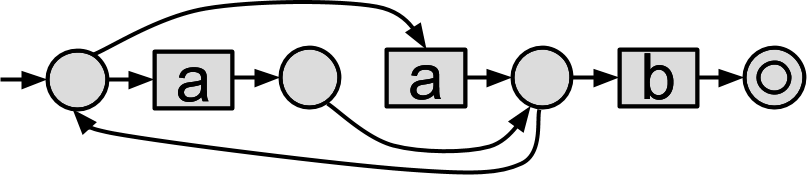
\includegraphics[scale=0.4]{figures/exemplo_automato_puro.png}
  \caption{Representação do autômato como diagrama de estados}
  \label{fig:exemplo_automato_puro}
\end{figure}


{
  \lstset{%
    basicstyle=\ttfamily\normalsize,
  }
\begin{lstlisting}[caption={Representação do autômato como array},label=lst:automaton_array]
	[(1, 3), 'a', (2,), 'a', (1, -4), 'b']
\end{lstlisting}
}

\noindent\begin{minipage}{\textwidth}
{
  \lstset{%
    basicstyle=\ttfamily\normalsize,
  }


\begin{lstlisting}[caption={Representação do autômato como instruções},label=lst:automaton_instr]
0000: JUMP (1, 3)
0001: CONSUME a
0002: JUMP (2,)
0003: CONSUME a
0004: JUMP (1, -4)
0005: CONSUME b
0006: MATCH!
\end{lstlisting}
}
\end{minipage}


\section{Simulação}

A simulação é executada pelos métodos \emph{matcher} e \emph{match} da classe \emph{Machine}. A diferença entre os dois é que o primeiro retorna um iterador que avalia o estado da execução do autômato para cada caractere da entrada. O segundo apenas retorna o resultado do match no final. Na implementação, o método \emph{match} utiliza o método \emph{matcher}, como mostra a Listagem~\ref{lst:match}.

\vspace{0.5cm}
\begin{lstlisting}[caption={Implementação do método \emph{match}},label=lst:match]
def match(self, string):
    return reduce(lambda answer, s: s[1], self.matcher(string), None)
\end{lstlisting}

O método implementado para a simulação do autômato é a \emph{simulação paralela}. Este método foi escolhido por combinar uma complexidade assintótica polinomial com uma facilidade de implementação razoável.

Como é costumeiro na implementação de expressões regulares, o match é realizado caso qualquer substring do input pertença à linguagem definida. O método de simulação paralela leva vantagem por necessitar de pouca alteração para suportar este modo de execução.

A implementação baseia-se em ciclos de consumo, onde um conjunto de estados iniciais passa simultâneamente por uma transição pelo mesmo caractere $c$ para um conjunto de estados sequentes.

Para representar os estados, utilizamos duas listas, A e B, que em todo momento representam respectivamente: o conjunto de estados \emph{de consumo} alcançados até o início da avaliação do caractere atual (A) e o conjunto de estados que a avaliação do caractere atual irá alcançar (B). Após a avaliação de cada caractere estas listas são invertidas. 

Cada estado nestas listas vem acompanhado da posição na string original onde o match começou. Esta informação é criada quando o estado inicial é colocado na lista para cada um dos caracteres. Ela é então copiada cada vez que o estado é resolvido e avança para seus sucessores. Na lista, o estado é representado por uma tupla $(start, j)$, onde $start$ representa a posição na entrada onde o match começou e $j$ é o índice do estado atual.

É importante ressaltar que um mesmo estado nunca entra na lista B duas vezes no mesmo ciclo de consumo. Esta verificação é efetuada pelo array V, que controla o índice do último caractere onde cada estado entrou na lista de estados. Inicialmente, esta lista está preenchida com valores -1.

Como apenas estados de consumo entram nas listas de estados para participar do ciclo de consumo (por razões óbvias), é preciso avaliar todos os estados de decisão antes do início do ciclo de consumo. 

A Listagem \ref{lst:addnext} mostra a implementação do método \emph{addnext} que adiciona estados à próxima lista de consumo (B), resolvendo recursivamente estados de decisão em seus respectivos próximos estados de consumo. Este método também retorna o número de vezes que o estado de aceite foi alcançado.

\vspace{0.5cm}
\begin{lstlisting}[caption={Implementação do método \emph{addnext}},label=lst:addnext]
def addnext(start, i, j):
    if j==self.n: return 1
    if V[j] == i: return 0
    V[j] = i

    if isinstance(self.states[j], tuple):
        return sum(addnext(start, i, j+k) for k in self.states[j])

    B.append((start, j))
    return 0
\end{lstlisting}

Assim, cada ciclo de consumo é marcado pelos passos:

\begin{itemize}
    \item Iniciar novo fluxo no estado inicial com o caractere atual.
    \item Inverter as listas de consumo, limpando a lista de próximo (B).
    \item Avaliar o consumo do caractere atual adicionando os estados subsequentes na lista de próximo.
\end{itemize}

A Listagem~\ref{lst:matcher} mostra a implementação destes passos. A linha 5 adiciona um novo fluxo começando no caractere $i$. As linhas 8 e 9 invertem as listas de consumo. Finalmente, as linhas 11-13 avaliam os estados de consumo contra a entrada, avançam os estados devidos, além de atualizar a melhor resposta, caso algum desses estados alcance o estado de aceite.

\vspace{0.5cm}
\begin{lstlisting}[caption={Implementação do método \emph{matcher}},label=lst:matcher]
def key(a): return (a[1]-a[0], -a[0]) if a else (0, 0)

answer = None
for i, c in enumerate(string):
    addnext(i, i, 0)
    yield i, answer, B
    
    A, B = B, A
    del B[:]

    for start, j in A:
        if self.states[j] in (None, c) and addnext(start, i+1, j+1):
            answer = max(answer, (start, i+1), key=key)
    
yield len(string), answer, B
\end{lstlisting}

\section{Visualização}

Valendo-se da implementação do método \emph{matcher} foi possível construir uma visualização em modo texto, passo-a-passo, da execução do algoritmo, que visa ajudar na compreensão. Trata-se de uma ferramenta de linha de comando (também escrita em Python) que utiliza o PyRex .

É possível chamar o visualizador com o comando \emph{./view.py (regex) (input)}, e.g.:

\begin{verbatim}
./view.py a+b+c+ aabbbcccc
\end{verbatim}

No exemplo, a execução do programa iria mostrar os passos do match desta expressão regular. O autômato gerado pode ser visualizado na Figura~\ref{fig:view_automaton}. Alguns passos da execução podem ser vistos nas Figuras~\ref{fig:exemplo_view_passo_3} e \ref{fig:exemplo_view_passo_6}.

\begin{figure}[!htbp]
  \centering
  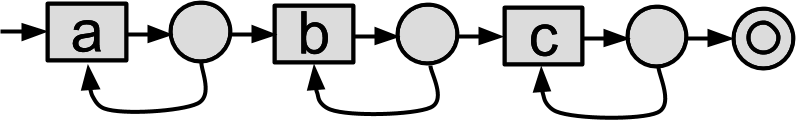
\includegraphics[scale=0.35]{figures/view_automaton.png}
  \caption{Autômato para expressão $a^+b^+c^+$}
  \label{fig:view_automaton}
\end{figure}

\begin{figure}[!htbp]
  \centering
\begin{verbatim}
Best answer: <none>
Input: aabbbcccc
          ^ (3)

  3 >0000: CONSUME a
     0001: JUMP (1, -1)
  0 >0002: CONSUME b
     0003: JUMP (1, -1)
  0 >0004: CONSUME c
     0005: JUMP (1, -1)
     0006: MATCH!
\end{verbatim}
  \caption{Exemplo de visualização lendo o 4º caractere da string}
  \label{fig:exemplo_view_passo_3}
\end{figure}

Esta forma de exibir mostra o estado atual de todos os fluxos sendo executados pelo autômato. O número exibido ao lado de cada instrução é o índice da entrada onde aquele fluxo começou. No exemplo específico, há três fluxos em execução: 

\begin{itemize}
\item{O que começa com cada caractere da string. (3)}
\item{O que continua lendo caracteres b da entrada, enquanto houver. (0)}
\item{O que está pronto para ler caracteres c, quando começarem. (0)}
\end{itemize}


\begin{figure}[!htbp]
  \centering
\begin{verbatim}
Best answer: aabbbc (0, 6)
Input: aabbbcccc
             ^ (6)

  6 >0000: CONSUME a
     0001: JUMP (1, -1)
     0002: CONSUME b
     0003: JUMP (1, -1)
  0 >0004: CONSUME c
     0005: JUMP (1, -1)
     0006: MATCH!
\end{verbatim}
  \caption{Exemplo de visualização lendo o 7º caractere da string}
  \label{fig:exemplo_view_passo_6}
\end{figure}

Neste momento, já existe um match para a string (visto que já existem caracteres c lidos). O melhor match até o momento é mostrado na linha \emph{Best answer}. Este valor é atualizado a cada passo. Além disso, os seguintes estados estão ativos:

\begin{itemize}
\item{O que começa com cada caractere da string. (6)}
\item{O que continua lendo caracteres c da entrada, enquanto houver. (0)}
\end{itemize}

A ferramenta utiliza o método matcher, que retorna um iterador que, a cada iteração, retorna uma tupla $(i, answer, state)$, onde $i$ é o índice atual que está sendo lido na entrada, $answer$ é a melhor resposta conseguida até o momento e $state$ é a lista de estados atuais, que é composta de várias tuplas $(start, j)$.

O código-fonte completo da ferramenta pode ser visto no Apêndice~\ref{app:view_source}.

%======================================================================================
\chapter{Análise dos Resultados}\label{cap:analysis}
%======================================================================================

Neste capítulo serão abordadas as principais diferenças entre a implementação proposta neste trabalho em comparação com outras implementações populares.

Algumas comparações com implementações específicas serão feitas, por isso, faz-se necessário definir claramente as caracteristicas e versões destas implementações. Segue uma tabela que clarifica tais questões:

\begin{center}
	\begin{tabular}{ c | c | c }
		{\bf Implementação} & {\bf Ambiente} & {\bf Linguagem original} \\
		\hline 
		pyrex & Python 2.7.3 & Python \\
		re & Python 2.7.3 & C \\
		Oniguruma & Ruby 1.9.3 & C \\
		java.util.regex & Java 1.6.0\_45 & Java \\
	\end{tabular}
\end{center}


\section{Retorno do Método \emph{match}}

O problema de reconhecer palavras usando expressões regulares é uma problema de \emph{decisão}. Isto significa que ele aceita apenas uma entre duas respostas: \emph{sim} ou \emph{não}. Entretanto, provou-se útil ao longo do tempo não só reconhecer palavras em linguagens regulares, mas também qualquer sub-palavra pertencente a ela, retornando, então, sua localização na palavra original.

Uma expressão regular $abcd$ retornaria um match válido numa palavra $zzabcdzz$. Este comportamento permite que múltiplas soluções sejam válidas. Por exemplo, a mesma expressão poderia encontrar dois resultados diferentes na palavra $abcdabcd$. Muitos resultados poderiam se sobrepor, inclusive. A expressão $a^*$, ao avaliar a palavra $aaaa$ pode levar a 10 resultados diferentes. A implementação utilizada influencia bastante na escolha de qual dos resultados deve ser retornado.

A implementação proposta neste projeto sempre favorece as respostas mais longas. Em caso de empate, é favorecida a resposta que inicie mais à esquerda na entrada. Este comportamento é garantido pela função \emph{key}, representada na Listagem~\ref{lst:matcher} na Página~\pageref{lst:matcher}.

Este comportamento é coerente com o artigo original de Thompson e, consequentemente, com as implementações de ferramentas como \emph{sed} e \emph{grep} do sistema operacional Unix. Por outro lado, diverge de outras implementações usuais baseadas na do Perl, que geralmente retornam a primeira resposta encontrada seguindo uma ordem gulosa de avaliação \cite{bib:Cox07}.

Uma forma fácil de verificar esta diferença é comparar o match da expressão \linebreak
$a^*(b|abc)$ contra a string $abc$. A implementação padrão do Python retornaria a string $ab$. A implementação neste projeto encontrará a string $abc$. A diferença é que a primeira tenta avaliar o máximo que pode na repetição $a^*$, enquanto a segunda consegue visualizar globalmente os matches possíveis.

\section{Reconhecimento de \emph{backreferences}: um problema NP-difícil}

No Capítulo~\ref{cap:theory} foram mostradas diversas formas de simular o autômato construído a partir da expressão regular. Cada uma delas tem características particulares de complexidade de tempo e espaço, além de dificuldades de implementação diversas.

O que se propõe nesta seção é demonstrar que qualquer implementação de expressões regulares que suporte \emph{backreferences} necessariamente torna o \emph{match} um problema NP-difícil. Este resultado mostra que qualquer algoritmo conhecido é suficientemente ineficiente para aplicações onde o tempo de execução é crítico.

\subsection{Problemas NP-difíceis}

A classe de problemas NP-difíceis (\emph{Non-deterministic Polynomial-time hard}) são aqueles para os quais existem problemas NP-completos redutíveis a eles em tempo polinomial. Nem todos os problemas em NP-difícil são de decisão, diferentemente dos problemas em NP.

A classe NP diz respeito a todos os problemas de \emph{decisão} que podem ser resolvidos em tempo polinomial em uma máquina de Turing não-determinística. Isto inclui também os problemas de decisão que podem ser resolvidos em máquinas de Turing determinísticas em tempo polinomial (conjunto P). Não há até o momento qualquer prova conclusiva se há algum problema em NP que não esteja também em P. Também não se sabe se todos os problemas de NP estão em P. A Figura \ref{fig:p_np} mostra como seria o diagrama de conjuntos em ambos os casos.


\begin{figure}[!htbp]
\centering
\begin{subfigure}{.5\textwidth}
  \centering
  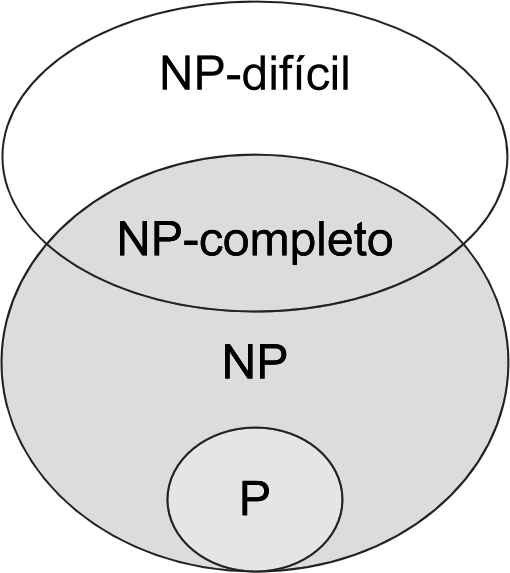
\includegraphics[scale=0.3]{figures/p_neq_np.png}
\end{subfigure}%
\begin{subfigure}{.5\textwidth}
  \centering
  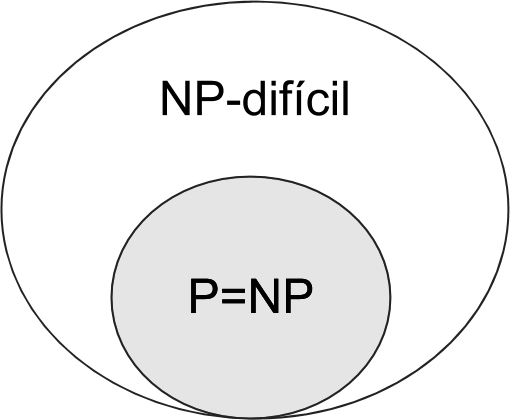
\includegraphics[scale=0.3]{figures/p_eq_np.png}
\end{subfigure}
\caption{Diagrama de conjuntos caso $P \neq NP$ e $P=NP$, respectivamente}
\label{fig:p_np}
\end{figure}


Uma característica importante dos problemas em NP é que se a resposta para o problema for \emph{sim}, dada um \emph{certificado} (ou \emph{testemunha}) que mostre tal fato, é possível determinar em tempo polinomial se esta resposta está correta ou não utilizando uma máquina de Turing determinística.

Nos anos 70, Stephen Cook introduziu o conceito de problemas NP-completos \cite{bib:Cook71}. São problemas em NP tais que qualquer outro problema em NP pode ser reduzido a eles em tempo polinomial. Qualquer solução polinomial de um problema NP-completo demonstraria que todos os problemas em NP podem ser resolvidos polinomialmente em máquinas de Turing determinísticas.

Cook também provou provou que o problema de satisfabilidade booleana ({\sc sat}) é NP-completo. Resultado parecido com o que Leonid Levin alcançou independentemente em 1973 \cite{bib:Levin73}. Hoje este resultado é conhecido como teorema de Cook--Levin. 

O problema de satisfabilidade consiste em determinar se existe uma interpretação que satisfaça uma expressão booleana, i.e. se existe uma atribuição de variáveis que avalie tal expressão como \emph{verdadeira}. Neste problema, o \emph{certificado} consiste no conjunto de valores a se atribuir às variáveis para que a expressão seja avaliada como verdadeira. Para verificá-la, basta substituir por tais valores e avaliar a expressão resultante.

Certas variações de {\sc sat} podem pertencer a classes de problemas diferentes. Uma variação possível é restringir às expressões booleanas a sempre estarem na CNF (\emph{Conjunctive Normal Form} ou Forma Normal Conjuntiva). 

Se a expressão booleana estiver escrita na 2CNF (forma normal conjuntiva com no máximo 2 variáveis por cláusula) este problema torna-se polinomial. Neste caso, é referido como 2-satisfabilidade ({\sc 2sat}). Entretanto, se a expressão estiver escrita na 3CNF, o problema ({\sc 3sat}) continua NP-completo \cite{bib:Karp72}.

Uma expressão está na 3CNF se ela está na forma:

\begin{equation*}
(A_{11} \lor A_{12} \lor A_{13}) \wedge (A_{21} \lor A_{22} \lor A_{23}) \wedge \cdots \wedge (A_{n1} \lor A_{n2} \lor A_{n3}),
\end{equation*}


onde $A_{ij}$ pode ser tanto uma variável ($X$) quanto a negação de uma variável ($\neg X$).

\subsection{Reconhecimento de \emph{backreferences}}

Durante o reconhecimento de expressões regulares, uma funcionalidade comum em implementações modernas é a capacidade de definir grupos de captura. Uma expressão $(a^+)(b^+)(c^+)$ teria quatro grupos de captura, numerados de 0 a 3. E o reconhecimento de uma string com esta expressão resultaria em uma tupla com o valor capturado por cada um dos grupos. A string $aabbbcccc$ resultaria nas capturas $(aa, bbb, cccc)$.

Baseado nesta funcionalidade, muitas implementações modernas adicionam a capacidade de referenciar tais grupos de captura ainda durante o match de uma string. Por exemplo, dada uma linguagem $L = \{a^nba^n \mid n \in \mathbb{N}\}$, seria possível denotá-la com a expressão $(a^*)b \backslash 1$. A referência ao grupo de captura 1 $(a*)$ se dá pela expressão $\backslash 1$.

Denotaremos aqui o problema de reconhecimento de expressões regulares com \emph{backreferences} como {\sc Match}.


\begin{definition}{Match}
Dada uma expressão regular $E$ com \emph{backreferences} abrangendo $n$ grupos de captura e $S$ a string a ser reconhecida, encontrar tupla $C = (c_1, c_2, \cdots, c_n)$, onde $c_i$ é substring de $S$ relativa ao reconhecimento do $i$-ésimo grupo de captura.
\end{definition}

\begin{theorem}
{\sc Match} é NP-difícil.
\end{theorem}
\begin{proof}
{\sc 3sat} é redutível para {\sc Match} utilizando a seguinte lógica: para resolver uma fórmula com $n$ variáveis e $m$ cláusulas, define-se a expressão regular

\setlength\abovedisplayskip{0pt}
\begin{equation*}
            E = 
                   \wedge (x?)^n .^*;
                   (?:\backslash 1v_{11}|\backslash 2 v_{12}|\backslash 3 v_{13}),
                   (?:\backslash 1v_{21}|\backslash 2 v_{22}|\backslash 3 v_{23}),                   
                   \ldots
                   (?:\backslash 1v_{m1}|\backslash 2 v_{m2}|\backslash 3 v_{m3}),                   
                    \$ 
\end{equation*}

\noindent e a string a ser reconhecida

\setlength\abovedisplayskip{0pt}
\begin{equation*}
S = x^n;x,^m
\end{equation*}

\noindent onde $v_{ij} = x$ se a variável $j$ da cláusula $i$ aparecer negada na fórmula, caso contrário, $v_{ij} = \epsilon$. Isto força o reconhecimento da \emph{backreference} $\backslash j$ como $x$ ou $\epsilon$ respectivamente, porém pelo menos uma das variáveis precisa reconhecer a substring $x,$ definida para cada cláusula na string $S$. Assim, existem grupos de captura $C = (c_1, c_2, \cdots, c_n)$ se e somente se for possível reconhecer tanto as expressões dos grupos de captura ($x$ ou $\epsilon$ para $verdadeiro$ ou $falso$, respectivamente), como as \emph{backreferences} que representam as cláusulas da fórmula de forma consistente. Como tanto a expressão $E$ quanto a string $S$ podem ser construídas em $O(n+m)$, {\sc Match} é NP-difícil. \qed
\end{proof}

\subsection{Implementação de {\sc 3sat} com expressões regulares}

Para exemplificar a demonstração da seção anterior, será descrita aqui uma implementação que permite a solução de instâncias do problema \textsc{3sat} utilizando as expressões regulares da linguagem Python.

Como exemplo, pode-se observar a fórmula:

\setlength\abovedisplayskip{0pt}
\begin{equation*}
(x_1 \lor x_2 \lor \neg x_3) \wedge 
(x_1 \lor \neg x_2 \lor x_3) \wedge
(\neg x_1 \lor \neg x_2 \lor x_3) \wedge 
(\neg x_1 \lor \neg x_2 \lor \neg x_3).
\end{equation*}

É possível construir uma expressão regular que represente esta expressão, e.g.

\setlength\abovedisplayskip{0pt}
\begin{equation*}
\wedge (x?)(x?)(x?).^*;
                   (?:\backslash 1|\backslash 2|\backslash 3x),
                   (?:\backslash 1|\backslash 2x|\backslash 3),
                   (?:\backslash 1x|\backslash 2x|\backslash 3),
                   (?:\backslash 1x|\backslash 2x|\backslash 3x), \$
\end{equation*}

Ao tentar realizar match desta expressão com a string $xxx;x,x,x,x,$ o resultado será a tupla de strings $(`x', `', `x')$, denotando que caso $x_1 = verdadeiro, x_2 = falso, x_3 = verdadeiro$, a expressão original será satisfeita.

A primeira parte da expressão denota os grupos iniciais onde entre 0 e 3 variáveis podem ser verdadeiras (reconhecendo `x'). A segunda parte da expressão define as cláusulas. Toda cláusula começa com a definição de um grupo que não gera captura, $(?:\ldots$. Então cada variável é descrita com uma altenação. $\backslash i$ referencia a variável $x_i$, enquanto $\backslash ix$ denota sua negação.

A Listagem~\ref{lst:nphard} mostra uma implementação em Python de {\sc 3sat} utilizando expressões regulares.

\vspace{0.5cm}
\lstinputlisting[caption={Implementação de {\sc 3sat} com expressões regulares},label=lst:nphard]{benchmark/nphard.py}

\section{Benchmarks}

Apesar do match de \emph{backreferences} ser um problema NP-difícil, match de expressões regulares por si só não é. O principal objetivo neste trabalho é mostrar que mesmo em casos onde as expressões poderiam ser avaliadas em tempo polinomial, elas não o são em uma grande parte de implementações modernas.

Para demonstrar este ponto, foram feitos alguns testes utilizando a mesma expressão regular em diversas implementações e comparando seus tempos de execução em relação ao crescimento da string de entrada. O código-fonte de todos os testes pode ser encontrado no Apêndice~\ref{app:benchmarks_source}. Todas as tabelas de valores podem ser encontradas no Apêndice~\ref{app:benchmarks_tables}.

Todos os gráficos estão em escala logarítmica, para facilitar a visualização do grande intevalo de valores que cada implementação representa.

\subsection{Benchmark 1: (a?a)+b}

Neste teste a string $a^n$ foi avaliada contra a expressão regular $(a?a)^+b$. O objetivo é mostrar o comportamento exponencial de implementações baseadas em backtracking. A expressão escolhida força a escolha para cada caractere da entrada sobre usar ou não o caractere $a$ na expressão $a?$. 

A Figura~\ref{fig:graph_bench_1} mostra o tempo de execução para as diferentes implementações. A tabela na Seção~\ref{sec:table_bench_1} (Página~\pageref{sec:table_bench_1}) contém os dados para este gráfico.

\begin{figure}[!htbp]
\centering
\begin{tikzpicture}
	\begin{semilogyaxis}[xlabel=n, ylabel=tempo (s), legend columns=5, cycle list name=black white]
	\addplot table[x=n,y=pyrex] {benchmark/bench1.txt};
	\addplot table[x=n,y=python] {benchmark/bench1.txt};
	\addplot table[x=n,y=ruby] {benchmark/bench1.txt};
	\addplot table[x=n,y=java] {benchmark/bench1.txt};
	\legend{pyrex, python, ruby, java}
	\end{semilogyaxis}
\end{tikzpicture}
\caption{Tempo de execução (em escala logarítmica) para match de $a^n$ contra $(a?a)^+b$}
\label{fig:graph_bench_1}
\end{figure}

Um ponto interessante a ser observado é que a implementação em Java, que inicialmente tem a pior constante de todas, rapidamente sofre compilação JIT (\emph{Just in Time}), que faz com que o tempo de execução caia bastante, porém mantendo seu caráter exponencial.

\subsection{Benchmark 2: a*b}

Neste teste, o objetivo era demonstrar a alta constante da implementação PyRex em casos onde o tempo de execução é linear para todas as implementações.

A Figura~\ref{fig:graph_bench_2} mostra o tempo de execução para as diferentes implementações. A tabela na Seção~\ref{sec:table_bench_2} (Página~\pageref{sec:table_bench_2}) contém os dados para este gráfico.

\begin{figure}[!htbp]
\centering
\begin{tikzpicture}
	\begin{semilogyaxis}[xlabel=n, ylabel=tempo (s), legend columns=5, cycle list name=black white]
	\addplot table[x=n,y=pyrex] {benchmark/bench2.txt};
	\addplot table[x=n,y=python] {benchmark/bench2.txt};
	\addplot table[x=n,y=ruby] {benchmark/bench2.txt};
	\addplot table[x=n,y=java] {benchmark/bench2.txt};
	\legend{pyrex, python, ruby, java}
	\end{semilogyaxis}
\end{tikzpicture}
\caption{Tempo de execução (em escala logarítmica) para match de $a^n$ contra $a^*b$}
\label{fig:graph_bench_2}
\end{figure}

É possível observar uma clara desvantagem de implementações em código gerenciado (PyRex e Java) contra outras implementações escritas em C (Ruby e Python) para casos onde a complexidade de tempo é linear.

\subsection{Benchmark 3: a*a*a*a*a*b}

Neste teste, o objetivo era demonstrar como mesmo em casos onde implementações baseadas em backtracking não geram tempos de execução exponenciais, ainda assim é possível alcançar tempos de execução maiores que $O(n)$. Esta expressão força um backtracking para consumo de várias repetições $a^*$. O tempo de execução esperado para implementações baseadas em backtracking é $O(n^5)$.

A Figura~\ref{fig:graph_bench_3} mostra o tempo de execução para as diferentes implementações. A tabela na Seção~\ref{sec:table_bench_3} (Página~\pageref{sec:table_bench_3}) contém os dados para este gráfico.

\begin{figure}[!htbp]
\centering
\begin{tikzpicture}
	\begin{semilogyaxis}[xlabel=n, ylabel=tempo (s), legend columns=5, cycle list name=black white]
	\addplot table[x=n,y=pyrex] {benchmark/bench3.txt};
	\addplot table[x=n,y=python] {benchmark/bench3.txt};
	\addplot table[x=n,y=ruby] {benchmark/bench3.txt};
	\addplot table[x=n,y=java] {benchmark/bench3.txt};
	\legend{pyrex, python, ruby, java}
	\end{semilogyaxis}
\end{tikzpicture}
\caption{Tempo de execução (em escala logarítmica) para match de $a^n$ contra $a*a*a*a*a*b$}
\label{fig:graph_bench_3}
\end{figure}

Este resultado mostra ainda como certas otimizações estáticas permitem que a implementação do Ruby mantenha seu tempo de execução linear enquanto a implementação do Python, que também é escrita em C, tenha uma complexidade de tempo maior que a do PyRex.

%======================================================================================
\chapter{Conclusão}
%======================================================================================

\section{Contribuição}

A principal contribuição neste trabalho foi uma implementação didática de expressões regulares utilizando o método de construção de Thompson. Nela foi utilizada uma forma simples de representar os estados do autômato finito não-determinístico como instruções de uma máquina abstrata que pode ser implementada em qualquer plataforma. A implementação foi feita em Python para fins de simplicidade e didática.

Os resultados alcançados foram bastante satisfatórios, mostrando que é possível implementar expressões regulares com algoritmos polinomiais. A implementação, apesar de não ser a mais eficiente para casos triviais, mostrou-se muito útil para demonstrar didaticamente a teoria apresentada no Capítulo~\ref{cap:theory}.

No Capítulo~\ref{cap:analysis} mostrou-se com sucesso que o problema reconhecimento de expressões regulares com \emph{backreferences} é NP-difícil; mostrou-se também a incapacidade de implementações em linguagens como Python, Ruby e Java de reconhecê-las em tempo polinomial, mesmo para expressões sem \emph{backreferences}.

Estes resultados confirmam a necessidade de parcimônia ao utilizar expressões regulares, principalmente em softwares que compartilham recursos de hardware entre vários usuários, e.g. sites e outros serviços de rede.

\section{Funcionalidades não implementadas}

O principal objetivo neste trabalho era apresentar uma implementação simples de expressões regulares, algumas funcionalidades comuns em implementações modernas foram propositalmente ignoradas. Enquanto algumas delas podem ser implementadas facilmente sem sacrificar complexidade de tempo, outras necessariamente tornariam o match exponencial. A seguir são comentadas algumas funcionalidades não implementadas.

\begin{description}
	\item[Classes de caracteres:] Para facilitar a escrita de expressões, muitas implementações disponibilizam conjuntos pré-definidos de caracteres. Exemplos incluem $\backslash w$, que inclui letras, números e underscore; ou $\backslash d$, que inclui todos os caracteres numéricos. Também deveria ser possível reconhecer classes customizadas, e.g. $[0-9a-fA-F]$, para caracteres aceitáveis num número na base hexadecimal.

	\item[Suporte a Unicode:] Uma implementação moderna de expressões regulares precisa dar suporte a strings Unicode. Apesar de não mudar a complexidade de execução do algoritmo, a implementação precisa ter cuidado com muitos detalhes, e.g. a definição do que é um caractere aceitável numa palavra ($\backslash w$) varia conforme a codificação.

	\item[Captura de grupos:] A possibilidade de capturar grupos pode ser importante para extrair informações de strings. Por exemplo, para capturar números separados por vírgula, seria possível escrever a expressão $(\backslash d^+),(\backslash d^+)$. Assim, a primeira captura seria o primeiro número e a segunda o segundo número.

	\item[Repetições contadas:] É util poder definir a repetição de um certo grupo de captura um número finito de vezes, e.g. a expressão $a\{2,4\}$ deve reconhece exatamente as strings $aa$, $aaa$ e $aaaa$. É uma funcionalidade de simples implementação usando autômatos, bastando por exemplo reescrever a expressão como $aaa?a?$. Esta reescrita, porém, pode ter um crescimento exponencial. Um exemplo é a expressão $a\{1000000\}$. Onde uma expressão com 10 caracteres geraria um autômato com no mínimo um milhão de estados.
	
	\item[\emph{Zero-width assertions}:] Algumas vezes pode ser necessário condicionar o match de um grupo ao match de outras strings em volta da região do match principal. Exemplos incluem o match de fronteiras de palavra ($\backslash b$), que pode ser útil ao buscar por uma palavra inteira numa string. A expressão $\backslash bpalavra\backslash b$, por exemplo, procura por $palavra$ na entrada desde que não seja uma substring de nenhuma outra palavra.
	
	\item[\emph{Backreferences}:] Como já mencionado no Capítulo~\ref{cap:analysis}, \emph{backreferences} são a capacidade de referenciar outros grupos de captura. Foi provado também que esta funcionalidade torna o match um problema NP-difícil.
		
\end{description}


\section{Trabalhos Futuros}

A implementação apresentada no Capítulo~\ref{cap:implementation} abordou os pontos mais básicos do reconhecimento de expressões regulares. Devido à alta densidade de funcionalidades em implementações modernas de expressões regulares, uma nova implementação precisaria resolver outros problemas, antes de ser útil para a industria.

Nesta seção serão discutidas propostas de trabalhos futuros que podem dar continuidade à implementação apresentada, de forma a torná-la apta ao uso em programas comerciais.

\begin{description}
	\item[Reimplementar a máquina em C:] Uma das vantagens de descrever a expressão regular como instruções de uma máquina abstrata é a capacidade de implementá-la facilmente em qualquer linguagem. Durante os benchmarks, um dos pontos mais visíveis foi a desvantagem de uma implementação puramente em Python ao competir com outras implementações em C nos casos mais triviais. Uma proposta de novo trabalho seria reimplementar esta máquina de execução utilizando uma linguagem de mais baixo nível.
	
	\item[Implementar funcionalidades comuns:] Certas funcionalidades presentes em implementações modernas permitem uma representação mais concisa de certas linguagens sem sacrificar a complexidade de tempo do algoritmo. Alguns exemplos notáveis incluem: captura de grupos (sem \emph{backreferences}); alguns tipos de \emph{zero-width assertions}, como \$ ou $\backslash b$.
	
	\item[Realizar um mapeamento completo de funcionalides:] Ao longo do tempo, as funcionalidades em implementações expressões regulares começaram a divergir entre as diversas implementações desenvolvidas. Cada biblioteca implementa uma certa porção utilizando um certo algoritmo. Uma proposta de trabalho seria mapear todas essas funcionalidades, catalogando seu impacto na complexidade dos algoritmos que as implementam.
	
	
\end{description}

\backmatter


\appendix

\postextualchapter{Código-fonte da Biblioteca PyRex}\label{app:full_source}

\lstinputlisting[caption={Código-fonte da biblioteca PyRex},label=lst:fill_appendice]{pyrex/pyrex.py}

\postextualchapter{Código-fonte do Visualizador}\label{app:view_source}

\lstinputlisting[caption={Código-fonte do Visualizador},label=lst:view_appendice]{pyrex/view.py}

\postextualchapter{Código-fonte dos Benchmarks}\label{app:benchmarks_source}

\lstinputlisting[caption={Benchmark 1: (a?a)+b}, language=bash]{benchmark/bench1}

\lstinputlisting[caption={Benchmark 2: a*b}, language=bash]{benchmark/bench2}

\lstinputlisting[caption={Benchmark 3: a*a*a*a*a*b}, language=bash]{benchmark/bench3}

\lstinputlisting[caption={Benchmark runner}, language=bash]{benchmark/bench_run}

\lstinputlisting[caption={Benchmark com PyRex}]{benchmark/bench_pyrex}

\lstinputlisting[caption={Benchmark com Python}]{benchmark/bench_python}

\lstinputlisting[caption={Benchmark com Ruby}, language=ruby]{benchmark/bench_ruby}

\lstinputlisting[caption={Benchmark com Java (compilador)}, language=bash]{benchmark/bench_java}

\lstinputlisting[caption={Benchmark com Java (fonte)}, language=java]{benchmark/java_source.java}

\postextualchapter{Tabelas dos Benchmarks}\label{app:benchmarks_tables}

\section{Benchmark 1: (a?a)+b}
\label{sec:table_bench_1}

\begin{center}
\pgfplotstabletypeset[
    precision=3,
    every head row/.style={after row=\hline},
    every last row/.style={after row=\hline},
    ]{benchmark/bench1.txt}
\end{center}

\newpage
\section{Benchmark 2: a*b}
\label{sec:table_bench_2}

\begin{center}
\pgfplotstabletypeset[
    precision=3,
    every head row/.style={after row=\hline},
    every last row/.style={after row=\hline},
    ]{benchmark/bench2.txt}
\end{center}

\newpage
\section{Benchmark 3: a*a*a*a*a*b}
\label{sec:table_bench_3}

\begin{center}
\pgfplotstabletypeset[
    precision=3,
    every head row/.style={after row=\hline},
    every last row/.style={after row=\hline},
    ]{benchmark/bench3.txt}
\end{center}


\bibliography{bibliografia}

\end{document}

